% !TEX program = xelatex
% Standalone Appendix X
% Compact-object time-domain science with R=5000 slitless spectroscopy.

\documentclass[10pt,onecolumn]{article}

\usepackage[a4paper,margin=18mm,top=17mm,bottom=18mm]{geometry}
\usepackage{microtype}
\usepackage{amsmath,amssymb}
\usepackage{siunitx}
\usepackage{booktabs}
\usepackage{tabularx}
\usepackage{array}
\usepackage{longtable}
\usepackage{graphicx}
\graphicspath{{appendix_x_assets/}}
\usepackage[dvipsnames,svgnames,table]{xcolor}
\usepackage[most]{tcolorbox}
\usepackage{titlesec}
\usepackage{enumitem}
\usepackage{fancyhdr}
\usepackage{hyperref}
\usepackage{caption}
\usepackage{float}
\usepackage{tikz}
\usetikzlibrary{arrows.meta,calc,positioning,shapes.geometric,fit}

\definecolor{ink}{HTML}{151B23}
\definecolor{titlebg}{HTML}{5A284A}
\definecolor{softink}{HTML}{263441}
\definecolor{muted}{HTML}{5C6875}
\definecolor{paper}{HTML}{F7F6F2}
\definecolor{panel}{HTML}{FFFFFF}
\definecolor{line}{HTML}{D8DEE5}
\definecolor{teal}{HTML}{007C77}
\definecolor{blue}{HTML}{245AA6}
\definecolor{gold}{HTML}{B86B00}
\definecolor{rose}{HTML}{A7354D}
\definecolor{violet}{HTML}{5A4CA0}
\definecolor{orange}{HTML}{B55220}

\hypersetup{
  colorlinks=true,
  linkcolor=blue,
  citecolor=teal,
  urlcolor=gold,
  pdftitle={Appendix X: Compact-Object Time-Domain Science},
  pdfauthor={Juhan Kim}
}

\pagestyle{fancy}
\fancyhf{}
\fancyhead[L]{\sffamily\footnotesize 3.5-meter Segmented-Mirror Robotic Space Telescope}
\fancyhead[R]{\sffamily\footnotesize Appendix X: Compact Objects}
\fancyfoot[C]{\sffamily\footnotesize X-\thepage}
\renewcommand{\headrulewidth}{0.35pt}

\titleformat{\section}{\sffamily\Large\bfseries\color{ink}}{\thesection}{0.6em}{}
\titleformat{\subsection}{\sffamily\large\bfseries\color{violet}}{\thesubsection}{0.6em}{}
\titleformat{\subsubsection}{\sffamily\normalsize\bfseries\color{softink}}{\thesubsubsection}{0.6em}{}
\titlespacing*{\section}{0pt}{1.1em}{0.45em}
\titlespacing*{\subsection}{0pt}{0.85em}{0.3em}
\captionsetup{font={small,sf},labelfont={bf,color=violet}}
\setlist[itemize]{leftmargin=*,itemsep=2pt,topsep=3pt}
\setlist[enumerate]{leftmargin=*,itemsep=2pt,topsep=3pt}
\renewcommand{\arraystretch}{1.18}
\renewcommand{\thesection}{X.\arabic{section}}
\renewcommand{\thesubsection}{X.\arabic{section}.\arabic{subsection}}
\renewcommand{\thesubsubsection}{X.\arabic{section}.\arabic{subsection}.\arabic{subsubsection}}
\renewcommand{\thefigure}{X.\arabic{figure}}
\renewcommand{\thetable}{X.\arabic{table}}
\renewcommand{\theequation}{X.\arabic{equation}}
\newcolumntype{Y}{>{\raggedright\arraybackslash}X}
\newcolumntype{C}[1]{>{\centering\arraybackslash}m{#1}}
\newcolumntype{P}[1]{>{\raggedright\arraybackslash}p{#1}}
\newcommand{\topcell}[1]{\begin{minipage}[t]{\linewidth}\vspace{0pt}#1\end{minipage}}
\emergencystretch=3em

\newtcolorbox{leadbox}[1]{
  enhanced,
  colback=paper,
  colframe=#1,
  coltext=ink,
  boxrule=0.9pt,
  arc=2mm,
  left=2.2mm,right=2.2mm,top=1.8mm,bottom=1.8mm
}
\newtcolorbox{resultbox}[1]{
  enhanced,
  colback=white,
  colframe=#1,
  coltext=ink,
  boxrule=0.75pt,
  arc=1.5mm,
  left=2mm,right=2mm,top=1.6mm,bottom=1.6mm
}

\newcommand{\facility}{3.5-meter Segmented-Mirror Robotic Space Telescope}
\newcommand{\Rpoint}{R_{\rm point}}
\newcommand{\kms}{\mathrm{km\,s^{-1}}}
\newcommand{\micron}{\,\mu\mathrm{m}}

\begin{document}
\thispagestyle{empty}

\begin{tcolorbox}[enhanced,colback=titlebg,colframe=titlebg,arc=2.5mm,
  left=5mm,right=5mm,top=7mm,bottom=7mm]
{\sffamily\color{white}\fontsize{23}{28}\selectfont\bfseries
Appendix X: Compact-Object Time-Domain Science}\\[2.2mm]
{\sffamily\color{white}\fontsize{14}{18}\selectfont
with $R=5000$ slitless spectroscopy}\\[3mm]
{\sffamily\color{white!80}\normalsize
Neutron-star and black-hole transients, white dwarfs, and dwarf novae}
\end{tcolorbox}

\begin{leadbox}{violet}
\textbf{Central design claim.}
The compact-object program uses the point-source resolving power of a
space-based slitless spectrograph. The baseline wavelength range is
$0.2$--$1.5\micron$ and the point-source resolving power is
$\Rpoint=5000$, corresponding to approximately $60\,\kms$ per resolution
element. The native sampling resolves accretion-disk and wind profiles. The
same spectra may be binned when broad and faint transient features do not
require the native resolution. The time-domain experiment combines this
spectral information with rapid target-of-opportunity observations and
high-cadence imaging. Mid-infrared imaging is not part of the adopted
compact-object baseline.
\end{leadbox}

\vspace{2mm}
\noindent
\begin{tabularx}{\textwidth}{@{}P{38mm}Y@{}}
\topcell{\bfseries\color{violet}Baseline mode} &
\topcell{Point-source slitless spectroscopy with $R=5000$, supplemented by
multi-band imaging and high-cadence time series.}\\
\topcell{\bfseries\color{violet}Primary science} &
\topcell{Rapid optical and near-infrared follow-up of gravitational-wave
counterparts, plus accretion-disk spectroscopy of white dwarfs, neutron
stars, black holes, and dwarf novae.}\\
\topcell{\bfseries\color{violet}What is measured} &
\topcell{Line centroids, widths, asymmetries, equivalent widths, continuum
color, fading rate, orbital modulation, and spectral evolution.}\\
\topcell{\bfseries\color{violet}What is not claimed} &
\topcell{The telescope does not measure X-rays or gamma rays. A single
optical/NIR spectrum does not determine a neutron-star equation of state
without external gravitational-wave and radiative-transfer information.}
\end{tabularx}

\section{Science Scope and Instrument Logic}

The main proposal identifies compact objects as a scientific theme, but the
science case becomes testable only when each object class is connected to an
observable and a time requirement. The appendix makes the connection
explicit through three experiments. Rapid observations of merger counterparts
measure spectral evolution on a timescale of hours to days. Repeated spectra
of accreting binaries measure line profiles as a function of orbital phase and
accretion state. Uninterrupted imaging of white dwarfs measures pulsation
frequencies while a spectrum fixes the atmospheric state required by the
asteroseismic model.

Compact-object angular sizes are normally far below the diffraction scale.
An isolated target therefore retains the point-source resolution of the
slitless spectrograph. The result differs from the extended-galaxy case in
which morphology broadens the dispersed image. Point-like morphology does not,
however, remove spectral confusion. Each target produces a long trace and an
unrelated field source may overlap the trace. Direct imaging, a scene model
and more than one dispersion orientation remain part of the measurement.

The baseline is intentionally restricted to optical and near-infrared
observations. Kilonovae, accretion disks, dwarf novae, and polluted white
dwarfs all have diagnostic emission or absorption features in this range.
The instrument therefore does not require a mid-infrared detector to support
the core compact-object program. Infrared excess from cool dust is an
ancillary diagnostic that may be supplied by other facilities when needed.
The wavelength span is nevertheless a demanding instrumental requirement.
Ultraviolet efficiency, optical order control, near-infrared detector
performance, and cross-channel flux calibration must be demonstrated as
separate parts of the end-to-end design. A nominal wavelength interval alone
does not establish usable sensitivity throughout the interval.

For a point source, the resolving power gives
\begin{equation}
  \Delta\lambda = \frac{\lambda}{\Rpoint},
  \qquad
  \Delta v \simeq \frac{c}{\Rpoint}
  \simeq 60\,\kms.
  \label{eq:resolution}
\end{equation}
At H$\alpha$, the nominal resolution element is about $1.31$\,\AA.
The nominal scale does not imply that every line centroid is measured to
$60\,\kms$.
For a sufficiently bright and isolated line, centroid precision may be much
smaller than one resolution element. The limiting factor is then the photon
noise, calibration stability, line blending and the forward model of the
slitless scene.

The native resolving power serves different purposes for different source
classes. Cataclysmic-variable disk lines often span several hundred to more
than one thousand $\kms$. The line wings and double peaks are consequently
sampled by several resolution elements at $R=5000$. Kilonova ejecta instead
produce blended structures with characteristic velocities near a tenth of the
speed of light. The kilonova structures do not require $R=5000$ for detection.
The native pixels may be combined to obtain the continuum sensitivity required at
late epochs while the unbinned data retain narrow host-galaxy and foreground
features. The proposal must quantify this trade with spectra degraded to the
instrument line-spread function and injected into realistic backgrounds.

\begin{resultbox}{violet}
\textbf{Operational requirement.}
The spectroscopic program must preserve the point-source $R=5000$ mode for
compact objects. Binning to a lower resolution may be used for faint
continuum measurements, but the native data must retain the line-profile
information required for velocity, profile-asymmetry, and line-ratio studies.
\end{resultbox}

\section{Observables from \texorpdfstring{$R=5000$}{R=5000} Spectra}

The scientific value of the spectra is not a single redshift or a single
classification label. The scientific value lies in the joint time-dependent measurement of the
continuum and line structure. The forward model should report the following
quantities with a covariance matrix.

The covariance is essential because slitless extraction couples neighboring
wavelength bins and contaminating traces. A profile width obtained after
instrumental deconvolution is meaningful only when the wavelength solution,
line-spread function, and source position are fitted together. The same rule
applies to line ratios. Balmer ratios in an accretion disk depend on optical
depth and non-local thermodynamic equilibrium as well as extinction. The
Balmer decrement must therefore enter a disk-atmosphere model instead of being
used as an isolated reddening estimator.

\begin{table}[H]
\centering
\caption{Compact-object spectral observables and their physical interpretation.}
\label{tab:observables}
\begin{tabularx}{\textwidth}{@{}P{33mm}Y P{37mm}@{}}
\toprule
\textbf{Observable} & \textbf{Measurement} & \textbf{Physical use}\\
\midrule
Line centroid & Wavelength after wavelength calibration & Radial velocity,
redshift, orbital motion, ejecta velocity\\
FWHM and wings & Profile width after instrumental deconvolution & Disk
rotation, wind velocity, shock broadening\\
Double-peaked profile & Peak separation and asymmetry & Keplerian disk
kinematics and disk inclination constraints\\
Equivalent width & Line flux relative to local continuum & Ionization state,
accretion state, composition proxy\\
Balmer decrement & H$\alpha$/H$\beta$ and related ratios & Joint constraints
on optical depth, excitation, density, temperature, and extinction\\
He II and Bowen features & He II $\lambda4686$ and nearby blend & Hard
ionizing continuum and high-state accretion\\
Continuum slope & Multi-epoch spectral energy distribution & Temperature,
reddening, cooling, and disk contribution\\
Line evolution & Changes with time and orbital phase & Reprocessing,
outflow, disk instability, and transient classification\\
\bottomrule
\end{tabularx}
\end{table}

\section{Target Selection and Reference Samples}

The compact-object survey uses a tiered target-selection scheme. The scheme
combines a controlled reference sample with alert-driven observations and a
blind discovery channel. The reference sample supplies repeatable measurements
of line profiles and state changes. The alert channel captures short-lived
kilonovae and accretion episodes. Blind extraction searches the dispersed data
for compact emission-line sources that are absent from existing catalogs.

The initial selection is based on catalog classification, optical or X-ray
variability, orbital information, and expected spectral brightness. The
selection is refined after the ETC includes the measured throughput, zodiacal
background, detector configuration, and trace-overlap loss. The Ritter CV
catalog provides the initial dwarf-nova classification and subtype labels
\cite{rittercv}. LVK public alerts provide the kilonova trigger stream
\cite{lvkalerts}. A Target-of-Opportunity (ToO) observation is a rapid
follow-up observation initiated by such an alert.

\begin{table}[H]
\centering
\caption{Target-selection structure and reference observing plan. The exposure
times denote science integration across three roll angles. Slew, acquisition,
detector readout, and roll overhead are not included.}
\label{tab:target_selection}
\begin{tabularx}{\textwidth}{@{}P{31mm} P{42mm} P{38mm} Y@{}}
\toprule
\textbf{Sample} & \textbf{Selection} & \textbf{Reference exposure} &
\textbf{Campaign}\\
\midrule
Dwarf-nova intensive & Bright U Gem, SS Cyg, Z Cam, SU UMa, WZ Sge,
VW Hyi, and RU Peg with known orbital information & $3\times(300$--$600)$ s
per epoch & One year with monthly visits and 6--12 visits during each outburst\\
Dwarf-nova population & Catalogued U Gem, SU UMa, Z Cam, and WZ Sge systems
with measured or constrained brightness & $3\times(600$--$1200)$ s &
One visit every 4--6 weeks for 8--15 targets\\
KMTNet/KSP dwarf novae & Published dwarf novae discovered by the KMTNet
Supernova Program & Outburst exposures from $3\times300$ s to
$3\times1200$ s. Quiescent exposures are set by the ETC &
Regular visits for two recurrent systems and alert-driven visits for three
fainter or less frequent systems\\
AM CVn and ultracompact WD binaries & Helium emission, short orbital period,
or an established ultracompact classification & Phase bins shorter than
$0.1P_{\rm orb}$ with $1800$--$3600$ s total & Six to twelve months with
2--4 week state sampling and one phase-resolved sequence\\
UCXB benchmark & X-ray binaries with hydrogen-deficient or degenerate-donor
evidence & $2700$--$5400$ s total with phase-aware subexposures &
State-triggered visits over 6--12 months\\
WD plus NS or BH candidates & Gaia astrometric acceleration combined with
X-ray, UV, or radio evidence & $3\times(900$--$1800)$ s & Candidate confirmation
and two to four visits per year\\
Kilonova ToO & LVK BNS or NSBH alert with a visible counterpart and acceptable
solar elongation & $3\times(300$--$1200)$ s per epoch & Four epochs from 4 hr to
7 d after the alert\\
\bottomrule
\end{tabularx}
\end{table}

\begin{table}[H]
\centering
\caption{Initial compact-object candidate list. A benchmark label denotes a
well-studied system that calibrates the observing mode. A candidate label
denotes a system for which the nature of the donor or compact companion
remains part of the science case.}
\label{tab:compact_candidates}
\begin{tabularx}{\textwidth}{@{}P{34mm} P{72mm} Y@{}}
\toprule
\textbf{Class} & \textbf{Initial candidates} & \textbf{Use}\\
\midrule
Dwarf nova intensive & U Gem, SS Cyg, Z Cam, SU UMa, WZ Sge, VW Hyi, RU Peg &
Bright reference systems with complementary outburst behaviour\\
Dwarf nova population & RX And, SS Aur, ER UMa, YZ Cnc, OY Car, HT Cas,
VY Aqr, VW Vul & State changes, inclination effects, and population diversity\\
KMTNet/KSP dwarf novae & KSP-OT-201503a, KSP-OT-201611a, KSP-OT-201701a,
KSP-OT-201712a, KSP-OT-202104a & Ground-based discovery history combined
with regular and alert-driven space spectroscopy\\
AM CVn & AM CVn, HM Cnc, V407 Vul, ES Cet, HP Lib, CR Boo, V803 Cen, KL Dra,
GP Com, SDSS J1240$-$01, CE 315 & Helium accretion, orbital modulation, and
degenerate-donor diagnostics\\
UCXB benchmark & 4U 1820$-$30, 4U 1626$-$67, 4U 1916$-$05, 4U 0614+091,
4U 1543$-$624, 2S 0918$-$549, 4U 1850$-$087 & Hydrogen-deficient disks and
donor-composition constraints\\
WD plus NS or BH candidates & Gaia astrometric-acceleration candidates with
X-ray, UV, or radio counterparts & The list is generated from Gaia and
high-energy catalogs before the survey selection freeze\\
Kilonova reference event & GW170817 and AT2017gfo & ETC template and
multi-epoch spectral benchmark\\
Kilonova alert sample & Future LVK BNS and NSBH public alerts & ToO sample.
No fixed pre-survey object list is assumed\\
\bottomrule
\end{tabularx}
\end{table}

The candidate list is not a claim that every listed system contains a white
dwarf and a neutron-star or black-hole companion. The AM CVn and UCXB groups
include systems with degenerate-donor evidence and systems for which helium
stars remain possible. The WD plus NS or BH sample is intentionally defined by
observable selection criteria rather than by an unverified object list.

The shortest-period systems require a separate temporal design. HM~Cnc and
V407~Vul show modulations near 321 and 569 s. The UCXB 4U~1820$-$30 has an
orbital period near 685 s \cite{barros2007,stella1987}. A 600 s exposure
averages over a substantial fraction of an orbit and may erase the
velocity structure that motivates phase-resolved spectroscopy. The total
integration in Table~\ref{tab:target_selection} must be divided into short
subexposures for bright targets. Fainter systems provide a state-averaged
spectrum, but the resulting product must not be described as orbital
tomography.

The reference table also does not constitute a mission time allocation. The
annual charge is formulated as
\begin{equation}
 T_{\rm program} =
 \sum_k N_{{\rm target},k}N_{{\rm epoch},k}
 \left(t_{{\rm int},k}+t_{{\rm roll},k}+t_{{\rm read},k}\right)
 + T_{\rm slew}+T_{\rm ToO},
 \label{eq:time_budget}
\end{equation}
where the index $k$ denotes a source class. The roll and slew terms may exceed
the detector integration for bright dwarf novae. The final proposal must
evaluate Equation~\ref{eq:time_budget} with the spacecraft attitude model and
must rank the source classes before assigning a five-year yield.

\subsection{KMTNet/KSP dwarf-nova legacy sample}

The Korea Microlensing Telescope Network (KMTNet) operates three 1.6-m
wide-field telescopes in Chile, South Africa and Australia
\cite{kim2016kmtnet}. The longitude distribution supports nearly continuous
ground-based photometry when weather and seasonal visibility permit. The
KMTNet Supernova Program (KSP) has published five dwarf-nova discoveries with
measured light-curve histories or spectroscopic classifications
\cite{brown2018ksp,lee2019ksp,lee2022ksp,lee2024ksp,kim2026ksp}.

The five discoveries form a standing KMTNet/KSP legacy sample for the
spacecraft. Standing status does not imply a common observing interval.
Quiescent brightness and recurrence differ by several magnitudes and more
than an order of magnitude in time. Uniform sampling would spend excessive
time on KSP-OT-202104a in quiescence and would undersample the 6.6-day
activity of KSP-OT-201712a. Table~\ref{tab:ksp_dwarf_novae} assigns an initial
cadence tier from the published behaviour. The ETC and spacecraft visibility
model must set the final exposure and visit count.

\begin{table}[H]
\centering
\small
\caption{Published KMTNet/KSP dwarf novae proposed as a standing monitoring
sample. Coordinates use the J2000 reference frame. The cadence tiers are
initial observing assumptions rather than guaranteed mission allocations.}
\label{tab:ksp_dwarf_novae}
\begin{tabularx}{\textwidth}{@{}P{28mm} P{31mm} P{57mm} Y@{}}
\toprule
\textbf{Source} & \textbf{J2000 position} & \textbf{Published behaviour} &
\textbf{Proposed monitoring}\\
\midrule
KSP-OT-201503a \cite{brown2018ksp} &
$09^{\rm h}23^{\rm m}41.40^{\rm s}$\newline
$-21^\circ58^\prime09.5^{\prime\prime}$ &
U Gem-type candidate with $V\simeq17.3$ at maximum and $V\simeq22.6$ in
quiescence. The 2015 event lasted about 17 d. At least three events occurred
from 2011 to 2015. &
Tier 2. Observe every 3 to 4 weeks and begin daily spectroscopy after a
KMTNet rise alert. Follow the Balmer profile through the outside-in heating
front.\\
KSP-OT-201611a \cite{lee2019ksp} &
$06^{\rm h}42^{\rm m}02.1^{\rm s}$\newline
$-26^\circ00^\prime21.6^{\prime\prime}$ &
SU UMa or U Gem-type system with $V\simeq23.45$ in quiescence. A long
outburst and a short outburst were separated by about 91 d. The large
Galactic height makes the source a Population II candidate. &
Tier 2. Observe every 2 to 4 weeks within a seasonal campaign and increase
the cadence after an optical alert. Compare disk-line evolution between long
and short events.\\
KSP-OT-201701a \cite{lee2022ksp} &
$06^{\rm h}39^{\rm m}23.2^{\rm s}$\newline
$-26^\circ37^\prime18.8^{\prime\prime}$ &
Three superoutbursts and six normal outbursts were measured over 2.6 yr.
The normal cycle is about 76 d. The orbital period is
$51.91\pm2.50$ min. Strong double-peaked H~I and weak He~I emission are
present. &
Tier 1. Observe every 7 to 14 d and use daily visits during an outburst.
Measure peak separation, He~I/H$\alpha$ and the transition toward a
helium cataclysmic variable.\\
KSP-OT-201712a \cite{lee2024ksp} &
$07^{\rm h}24^{\rm m}07.70^{\rm s}$\newline
$-26^\circ19^\prime54.5^{\prime\prime}$ &
ER UMa-type system below the period minimum with a
$58.75\pm0.02$ min orbit. Outbursts recur every 6.6 d during standstills and
about every 15 d outside them. The spectrum contains double-peaked
H$\alpha$ and weak He~I. &
Tier 1. Observe every 2 to 3 d during focused 30 to 60 d windows. Resolve
line-profile changes across standstills and determine the response to the
high mass-transfer state.\\
KSP-OT-202104a \cite{kim2026ksp} &
$08^{\rm h}14^{\rm m}20.14^{\rm s}$\newline
$-26^\circ02^\prime37.21^{\prime\prime}$ &
Type D WZ Sge system with an amplitude near 8 mag and a 28.5 d outburst.
The superhump period is about 71.7 min. The measured brightness changes from
$V\simeq24.05$ in quiescence to $V\simeq16.01$ at maximum. &
Tier 3. Retain a low-cadence state check only when the ETC supports the
quiescent exposure. A KMTNet alert starts intensive spectroscopy within
12 hr and daily visits follow the early outburst.\\
\bottomrule
\end{tabularx}
\end{table}

KSP-OT-201712a and KSP-OT-201701a receive the regular allocation because
their recurrence times allow the mission to sample multiple disk states.
KSP-OT-201503a and KSP-OT-201611a retain a sparse baseline that establishes
the pre-outburst spectrum. KSP-OT-202104a is dominated by the alert mode
because its quiescent magnitude carries a high exposure cost while its
outburst remains bright for several weeks.

The $R=5000$ sequence links the KMTNet light curve to velocity-resolved
Balmer and helium profiles. The sequence measures disk peak separation,
profile asymmetry, line ratios and the change between quiescent emission and
outburst absorption. The KMTNet/KSP objects do not replace the bright
reference systems in Table~\ref{tab:compact_candidates}. The bright systems
measure instrumental repeatability while the KMTNet/KSP sample tests the
scientific reach at faint flux and unusual evolutionary state.

\subsection{KMTNet transient alerts and near-infrared spectroscopy}

An interface to KMTNet transient observations would provide a practical
external trigger for the compact-object program. The proposed notice supplies
a discovery time, a sky position and an optical light curve used to rank a
target before the spacecraft begins a spectroscopic visit. The notice does
not replace the space-based spectrum. The KMTNet observation identifies the
transient state while the space-based observation measures the spectral
response of the state.

The standalone appendix does not yet define the KMTNet/KSP alert performance.
The main proposal must supply the adopted field of view, filter set,
single-visit depth, revisit interval, astrometric uncertainty, classification
latency and annual duty cycle. The survey values determine whether KMTNet
discovers an outburst before the rise is complete and whether a kilonova
candidate is localized well enough for immediate spectroscopy. An alert link
without measured latency and sky coverage remains an interface concept rather
than a feasibility result.

Near-infrared spectroscopy is especially valuable for transient targets. The
reddest ejecta component of a kilonova may become dominant after the first
optical observations. Dust extinction is also weaker in the near-infrared than
in the optical. The $1.0$--$1.5\micron$ portion of the adopted band may therefore
follow a red component that is attenuated or missed at shorter wavelengths.
Space-based operation removes telluric absorption and provides a stable
background for repeated line-flux and continuum measurements. The same
near-infrared range contains Paschen and helium diagnostics that complement
the Balmer lines used for dwarf novae and accretion binaries.

The KMTNet/KSP notice supplies the position, discovery time, photometric
state and classification probability. The mission scheduler then evaluates
solar elongation, visibility duration, slew cost and the predicted spectral S/N.
A bright target receives an initial $3\times300$ s sequence. Later visits use
$3\times600$--$1200$ s when the source has faded. The number of roll angles
should be selected from the direct-image scene. Two orientations may be
sufficient for an isolated target while a crowded field may require a third.
The released product combines the KMTNet light curve with the calibrated
optical and near-infrared spectra.

The KMTNet link selects dwarf-nova outbursts, accretion-state changes and
optical counterparts of compact mergers. The space-based near-infrared
spectrum supplies information that a ground-based optical notice does not
provide. The proposed program should reserve ToO time for the alert stream in
addition to the standing KMTNet/KSP dwarf-nova sample.

The priority decision should use a reproducible score based on the probability
of the source class, the probability of spacecraft visibility, the predicted
S/N and the remaining lifetime of the transient state. A kilonova candidate
with a rapidly fading near-infrared prediction has a different time cost from
a dwarf nova that remains near maximum for several days. The alert service
must preserve the selection probabilities and provenance rather than distribute
only a binary target flag.

The most important distinction is between a line that is broad because the
gas is moving and a line that is broad because the source is extended along
the dispersion direction. Compact objects are advantageous because the
second effect is minimized. The reduction model must still propagate the point-spread
function, trace curvature, detector sampling, and overlap from unrelated
field sources in the same forward model.

The scene model must be tested with a transient that changes during the
sequence. A static contamination template may assign the variable flux to the
wrong trace when the target brightens between the direct image and dispersed
exposure. The simulation should include this temporal mismatch and should
report the recovered line flux as a function of target contrast, source
separation, and roll angle.

\section{Gravitational-Wave Counterparts}

\subsection{Binary neutron-star and neutron-star--black-hole mergers}

Binary neutron-star mergers provide the cleanest compact-object example of
why rapid space-based spectroscopy is useful. The gravitational-wave signal
constrains the binary masses, spins, distance, inclination and tidal
deformability. The electromagnetic counterpart supplies information about
the ejecta, viewing angle, host galaxy and radioactive heating. GW170817
demonstrated that the optical and near-infrared emission evolves on a
timescale of days and that different ejecta components may dominate at
different wavelengths \cite{abbott2017,arcavi2017,tanaka2017}.

The compact-object program does not require a mid-infrared channel for the
central measurement. The early blue component and the later redder
component are followed from the near-ultraviolet through the near-infrared
with repeated imaging and spectroscopy. The spectral sequence constrains
temperature evolution, expansion velocity, opacity and the relative
contribution of high- and low-electron-fraction ejecta. The identification of
strontium in the spectrum of GW170817 linked the kilonova directly to
nucleosynthesis rather than treating the event as a purely
photometric transient \cite{watson2019}.

The red wavelength limit defines the part of this experiment that the mission
performs alone. A lanthanide-rich component may peak beyond
$1.5\,\micron$ after the first few days. The adopted instrument measures the
blue component, the transition into the near-infrared and the short-wavelength
side of the red component. A claim about the full bolometric luminosity or the
late lanthanide-rich ejecta requires deeper infrared observations from another
facility. The proposal should quantify the information lost at the
$1.5\,\micron$ boundary with radiative-transfer templates instead of describing
the full red component as internally measured.

The broad ejecta spectrum also changes the role of the resolving power.
Kilonova features with velocities near $0.1c$ are strongly blended
\cite{pian2017,chornock2017}. Their detection is controlled mainly by
continuum S/N, wavelength coverage and response time. The $R=5000$ pixels
should be combined into lower-resolution spectral bins for ejecta inference.
The native data remain useful for a narrow host line, an intervening absorber,
or a contaminating field source. The observing mode must return both products
from one calibrated likelihood.

For each event, the inference must be joint. The measured data vector is
formulated as
\begin{equation}
  \boldsymbol{D}_{\rm KN} =
  \left\{F_\lambda(t),\,F_b(t),\,z_{\rm host},\,
  p(d_L,\iota\mid D_{\rm GW})\right\},
  \label{eq:kilonova_parameters}
\end{equation}
where $F_\lambda(t)$ is the spectral sequence and $F_b(t)$ denotes the
multi-band light curves. The host redshift is $z_{\rm host}$. The final term is
the gravitational-wave posterior for luminosity distance $d_L$ and inclination
$\iota$. A radiative-transfer model maps this data vector to the masses,
velocities, electron-fraction distributions and geometry of the dynamical
and wind ejecta. Opacity is wavelength dependent and evolves with ionization.
The opacity should not be treated as a single independent number without a
specified model. The telescope constrains the electromagnetic likelihood. The
nuclear equation of state enters only through joint inference with the
gravitational-wave posterior and merger simulations.

\begin{figure}[tp]
\centering
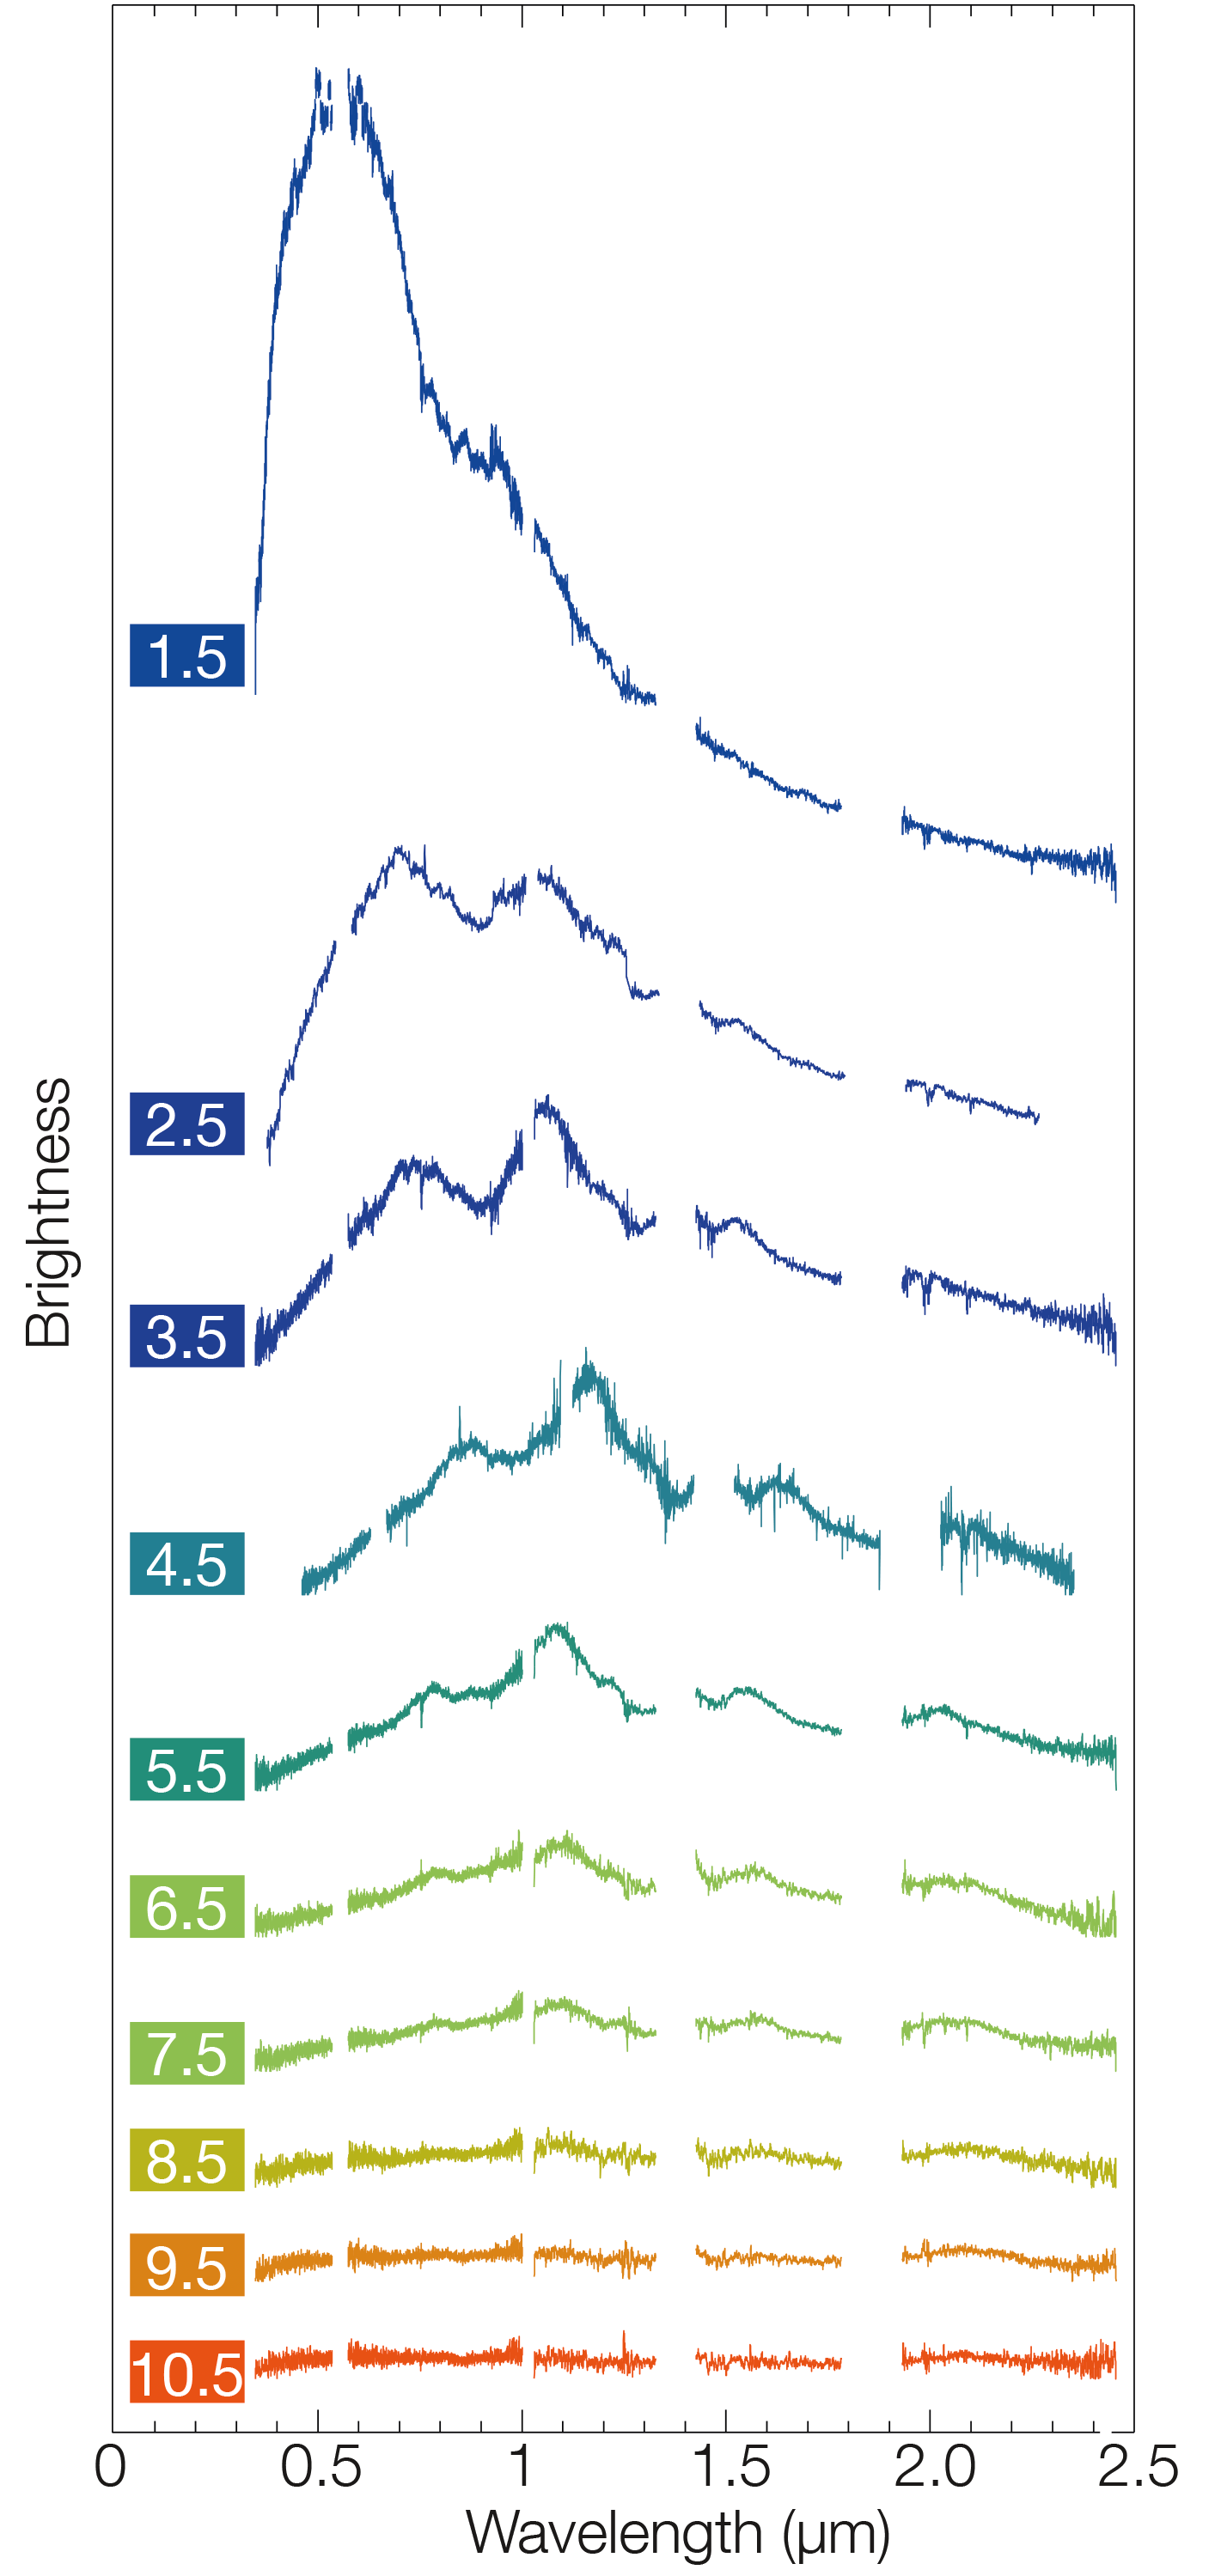
\includegraphics[width=0.95\textwidth,height=0.62\textheight]{gw170817_xshooter.png}
\caption{Actual observed optical and near-infrared spectra of the kilonova
AT~2017gfo associated with GW170817, obtained with the ESO VLT/X-shooter
instrument over twelve days. The sequence becomes progressively redder and
develops broad, evolving absorption structure, corresponding to the kilonova
rows in Table~\ref{tab:dwarf_lines}. The published reference montage extends
to about $2.5\,\micron$. The proposed baseline uses the $0.2$--$1.5\,\micron$
portion and does not require a mid-infrared mode. Reproduced from the ESO
public image archive \cite{eso1733j}. The physical interpretation is
discussed by Tanaka et al. (2017) and Watson et al. (2019)
\cite{tanaka2017,watson2019}.}
\label{fig:kilonova_observed}
\end{figure}

\subsection{ToO sequence and response requirement}

The proposed observing sequence is organized around the short-lived early
signal. A representative reference sequence is shown in Table~\ref{tab:too}.
The exact number of visits must be recomputed after the spacecraft slew,
solar-avoidance, and alert-localization simulations are complete.

The response clock should begin at the external alert time and should end at
the midpoint of the first science exposure. A spacecraft slew time alone
understates the latency because counterpart identification, command
authorization, guide-star acquisition and detector configuration occur
before useful photons are recorded. The first visit should use the minimum
number of roll angles supported by the direct-image scene. A mandatory
three-roll sequence may consume the interval in which the ultraviolet and blue
components change most rapidly.

\begin{table}[H]
\centering
\caption{Reference compact-object ToO sequence.}
\label{tab:too}
\begin{tabularx}{\textwidth}{@{}C{22mm} C{29mm} Y Y@{}}
\toprule
\textbf{Elapsed time} & \textbf{Mode} & \textbf{Primary information} & \textbf{Requirement}\\
\midrule
$<4$ hr & Imaging in several bands & Localization, color, counterpart ranking &
Rapid alert ingestion, slew, and acquisition\\
$4$--$12$ hr & $R=5000$ spectrum & Early line and continuum state &
Stable wavelength calibration and sufficient S/N per resolution element\\
$1$--$3$ d & Repeated spectroscopy & Ejecta velocity and ionization evolution &
Repeatable trace and flux calibration\\
$4$--$14$ d & Imaging plus spectroscopy & Cooling, recombination, and red component &
Low background and flexible queue scheduling\\
$>14$ d & Host and late-time imaging & Host redshift and transient subtraction &
Accurate reference imaging\\
\bottomrule
\end{tabularx}
\end{table}

The minimum mission-level requirement is not merely a fast slew. The alert
must pass through an end-to-end chain consisting of alert validation,
visibility calculation, dynamic scheduling, target acquisition, data-quality
assessment, and rapid dissemination. A response time that is fast at the
spacecraft but slow in the ground segment does not recover the early
kilonova signal.

The expected yield must be stated separately from the response goal. For an
observing interval $T$, the number of useful spectral sequences is formulated
as
\begin{equation}
 N_{\rm use}=T\int R_{\rm merger}(D)
 f_{\rm GW}(D)f_{\rm loc}(D)f_{\rm vis}
 f_{\rm id}f_{\rm S/N}(D)\,dV ,
 \label{eq:kilonova_yield}
\end{equation}
where $R_{\rm merger}$ is the merger rate density. The factors describe
gravitational-wave detection, useful localization, spacecraft visibility,
counterpart identification and adequate spectral S/N. Every factor depends
on the observing network and several depend on distance. The mission does not
replace this calculation with the number of public alerts. A credible
five-year estimate must quote the median yield and the uncertainty from the
merger-rate posterior.

\begin{figure}[H]
\centering
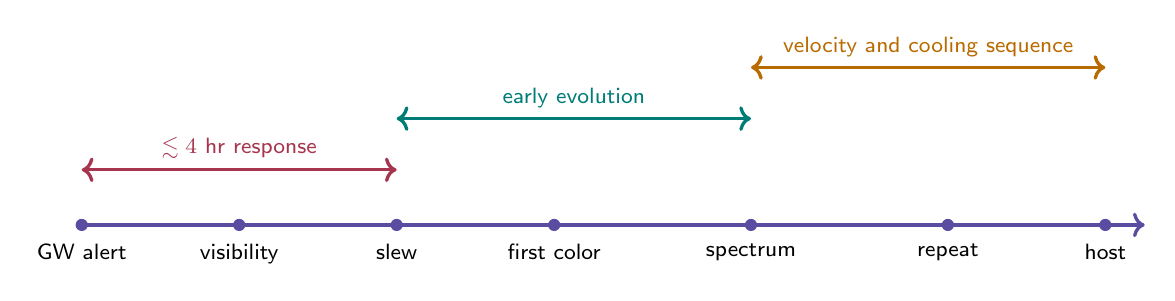
\begin{tikzpicture}[x=1cm,y=1cm,font=\sffamily\footnotesize]
  \draw[->,very thick,color=violet] (0,0) -- (13.5,0);
  \foreach \x/\t in {0/{GW alert},2/{visibility},4/{slew},6/{first color},8.5/{spectrum},11/{repeat},13/{host}} {
    \fill[violet] (\x,0) circle (2.2pt);
    \node[align=center,anchor=north] at (\x,-0.12) {\t};
  }
  \draw[<->,color=rose,line width=1.2pt] (0,0.7)--(4,0.7)
    node[midway,above] {$\lesssim4$ hr response};
  \draw[<->,color=teal,line width=1.2pt] (4,1.35)--(8.5,1.35)
    node[midway,above] {early evolution};
  \draw[<->,color=gold,line width=1.2pt] (8.5,2.0)--(13,2.0)
    node[midway,above] {velocity and cooling sequence};
\end{tikzpicture}
\caption{The compact-object ToO chain. The science requirement is a timed
sequence of measurements rather than a single rapid exposure.}
\label{fig:too_timeline}
\end{figure}

\section{Dwarf Novae and Cataclysmic Variables}

Dwarf novae are a particularly strong match to a robotic $R=5000$ slitless
spectrograph. Dwarf novae are compact, repeatedly variable and spectroscopically
rich. The standard disk-instability picture attributes dwarf-nova outbursts to a
thermal-viscous instability in the accretion disk of a close binary
\cite{warner1995,lasota2001}. The observed spectrum changes with accretion state.
Repeated spectra connect disk physics to the light curve and provide more
than a static classification.

\begin{figure}[H]
\centering
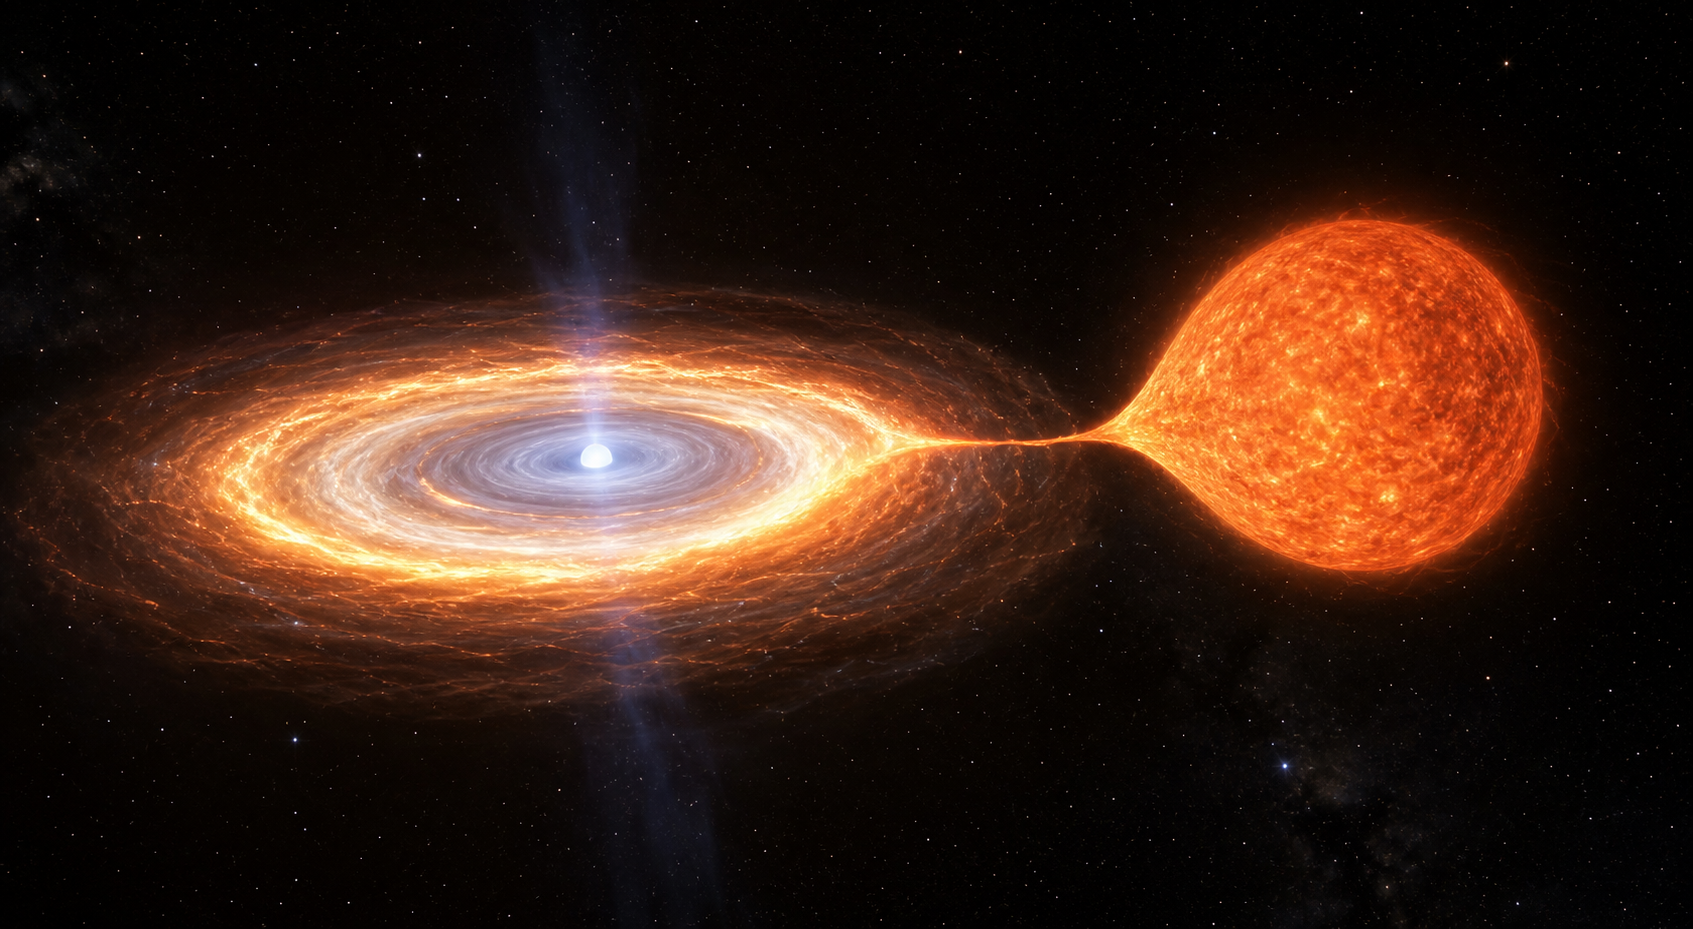
\includegraphics[width=0.94\textwidth]{dwarf_nova_typical_disk_outburst.png}
\caption{Artistic reconstruction of a typical dwarf-nova binary during a disk
outburst. A low-mass late-type donor transfers gas through the inner Lagrange
point to a white dwarf. The bright annulus represents a heating front moving
through the accretion disk. The image is a physical illustration rather than
an observed image.}
\label{fig:dwarf_nova_concept}
\end{figure}

\subsection{Where the outburst occurs}

The dwarf-nova outburst occurs in the accretion disk. The white dwarf remains
the compact central accretor, but the sudden optical brightening is not a
thermonuclear explosion on the white-dwarf surface. The distinction separates
a dwarf nova from a classical nova.

A typical system contains a white dwarf and a Roche-lobe-filling late-type
main-sequence donor. The donor loses gas through the inner Lagrange point.
The transferred gas carries angular momentum and forms a disk around the
white dwarf. The disk receives mass from the donor at a rate that may remain
below the rate required for a stable hot state.

The disk instability is a limit cycle rather than an explosion. Mass
accumulates while hydrogen is mostly neutral and angular-momentum transport is
inefficient. An annulus becomes thermally unstable when the surface density
crosses the critical value associated with partial hydrogen ionization. The
increased opacity and ionization move the annulus to the hot branch. A heating
front then travels through the disk and raises the inward mass flux. The
optical and ultraviolet continuum brightens as a larger disk area enters the
hot state. Depletion eventually permits a cooling front to form. The cooling
front returns the disk to the low-ionization branch and begins the next
quiescent interval.

The local thermal equilibrium has the familiar S-shaped relation between
surface density and effective temperature \cite{lasota2001}. The lower and
upper branches are stable over different surface-density intervals. The
middle branch near $6500$--$10{,}000$ K is unstable. The standard
parameterization uses a larger effective viscosity in the hot state than in
the cool state. The measurable rise and decay do not determine these
viscosities directly. Their interpretation requires a disk model in which the
thermal and viscous times are
\begin{equation}
 t_{\rm th}\sim \frac{1}{\alpha\Omega_{\rm K}},
 \qquad
 t_{\rm visc}\sim \frac{1}{\alpha\Omega_{\rm K}}
 \left(\frac{R}{H}\right)^2 ,
 \label{eq:disk_times}
\end{equation}
where $\alpha$ is the effective viscosity parameter, $\Omega_{\rm K}$ is the
Keplerian angular frequency and $H/R$ is the disk aspect ratio. A heating
front changes the local spectrum on a timescale closer to $t_{\rm th}$. The
redistribution of disk mass follows the longer viscous time. Spectra obtained
only at maximum light do not separate these processes.

An outside-in outburst begins in the outer disk when mass transfer and surface
density are high there. An inside-out event begins closer to the white dwarf
after the inner disk reaches the critical density. The propagation direction
changes the order in which the continuum, line wings, and peak separation
respond. A combined light curve and spectral sequence thereby tests the
front direction while constraining disk radius and mass-transfer state.

The optical rise does not mean that the white dwarf has exploded. The optical
luminosity comes mainly from the heated disk and from reprocessing on the
donor or the disk surface. Dwarf-nova spectra should consequently show a
transition from emission-line dominated quiescence to a brighter continuum
with broad absorption or mixed emission and absorption during outburst.
The U~Gem spectrum in Figure~\ref{fig:ugem_observed} provides a direct
observed example of the state dependence.

\subsection{Spectral features in the adopted wavelength range}

The optical and near-infrared range contains the principal diagnostics for
many dwarf novae.

\begin{table}[H]
\centering
\caption{Compact-object diagnostics available without a mid-infrared channel.
The dwarf-nova rows correspond to the observed U~Gem spectrum in
Figure~\ref{fig:ugem_observed}. The kilonova row corresponds to the observed
AT~2017gfo sequence in Figure~\ref{fig:kilonova_observed}.}
\label{tab:dwarf_lines}
\begin{tabularx}{\textwidth}{@{}P{28mm} P{37mm} Y@{}}
\toprule
\textbf{Feature} & \textbf{Typical use} & \textbf{Caveat}\\
\midrule
Balmer series & Disk temperature, optical depth, velocity field, extinction &
Profiles may switch from absorption to emission during outburst\\
H$\alpha$ & Strong time-series line and radial-velocity tracer &
May be contaminated by winds or the irradiated donor\\
He I lines & Ionization and disk-state indicator &
Several transitions are blended at low S/N\\
He II $\lambda4686$ & Hard ionizing component and high-state accretion &
Requires adequate blue sensitivity and calibration\\
Bowen blend near $4640$\,\AA & Reprocessed high-energy radiation and irradiated gas &
Blended components require forward profile fitting\\
Ca II infrared triplet & Cool dense gas and chromospheric or disk contribution &
Useful mainly for selected systems\\
Paschen lines & Near-infrared disk and wind diagnostics &
Telluric absorption is absent in space, which improves repeatability\\
Kilonova broad absorption complexes & Expansion velocity, temperature,
opacity and evolution of lanthanide-rich and lanthanide-poor ejecta &
Features are broad and blended. Interpretation requires radiative-transfer
models and the external gravitational-wave posterior\\
Kilonova continuum sequence & Cooling, recombination and radioactive-heating
timescale &
The early spectrum must be obtained quickly because the color evolves over
days\\
\bottomrule
\end{tabularx}
\end{table}

Figure~\ref{fig:ugem_observed} shows why the table must distinguish the
quiescent and outburst states. In quiescence, U~Gem has strong Balmer and
helium emission together with Ca~II emission and donor-star absorption bands.
Near outburst maximum, the continuum becomes much brighter and bluer, while
broad absorption features dominate and He~II may appear in emission. The
observed state change demonstrates that a time series of spectra follows
the disk-instability cycle rather than merely classify the object.

\begin{figure}[H]
\centering
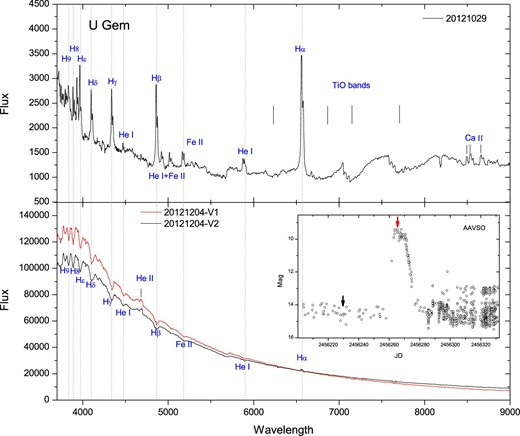
\includegraphics[width=0.83\textwidth]{ugem_lamost_spectrum.jpeg}
\caption{Actual observed spectra of the dwarf nova U~Gem from LAMOST. The
upper spectrum was obtained in quiescence and the lower spectra near the
2012 December outburst peak. The published labels identify Balmer lines,
He~I, He~II, Fe~II, TiO bands and the Ca~II infrared triplet. The labelled features
are the observed examples represented by the dwarf-nova rows in
Table~\ref{tab:dwarf_lines}. Reproduced from Zhi et al. (2020), Figure 1
\cite{zhi2020}.}
\label{fig:ugem_observed}
\end{figure}

The value of $R=5000$ is that the line profiles are resolved without making
the continuum survey prohibitively expensive. The nominal velocity scale is
about $60\,\kms$, while a high-S/N centroid or a phase-folded line profile
may yield a substantially smaller statistical uncertainty. The physically
interesting output is the profile as a function of orbital phase and
accretion state.

\subsection{Research enabled by the spectra}

The double-peaked profile provides the most direct disk-kinematic observable.
For an approximately Keplerian emitting disk, the peak separation scales as
\begin{equation}
 \Delta v_{\rm peak}\simeq
 2\left(\frac{GM_{\rm WD}}{R_{\rm em}}\right)^{1/2}\sin i ,
 \label{eq:double_peak}
\end{equation}
where $M_{\rm WD}$ is the white-dwarf mass, $R_{\rm em}$ is the characteristic
outer line-emitting radius and $i$ is the binary inclination
\cite{horne1986}. The high-velocity wings arise at smaller radii. A change in
peak separation does not by itself prove that the physical disk edge moved
because the emissivity distribution and optical depth also change during an
outburst. Multi-line fitting and an inclination prior are required.

The line and continuum sequence measures the accretion state in a
complementary way. Equivalent widths fall when a bright continuum dilutes an
emission line even if the line luminosity remains constant. Absolute
flux-calibrated line measurements are therefore required in addition to
equivalent widths. Blue-shifted absorption and asymmetric wings identify a
wind only when the same feature is reproduced at more than one roll angle and
is inconsistent with a contaminating trace. Balmer, helium, and Paschen
profiles then test whether the outflow changes with disk ionization.

Phase-resolved centroids measure the velocity of an irradiated donor or a
localized disk component. An emission-line velocity does not automatically
trace the white dwarf. The inferred semi-amplitude must be combined with
eclipse geometry, photometric ephemerides and a model for the emitting site.
The same analysis applied across rising, maximum and declining states tests
whether the disk-instability sequence predicts the observed front propagation
and line-forming radius. A population sample then relates the state sequence
to orbital period, recurrence time, and secular mass-transfer rate.

\begin{figure}[tp]
\centering
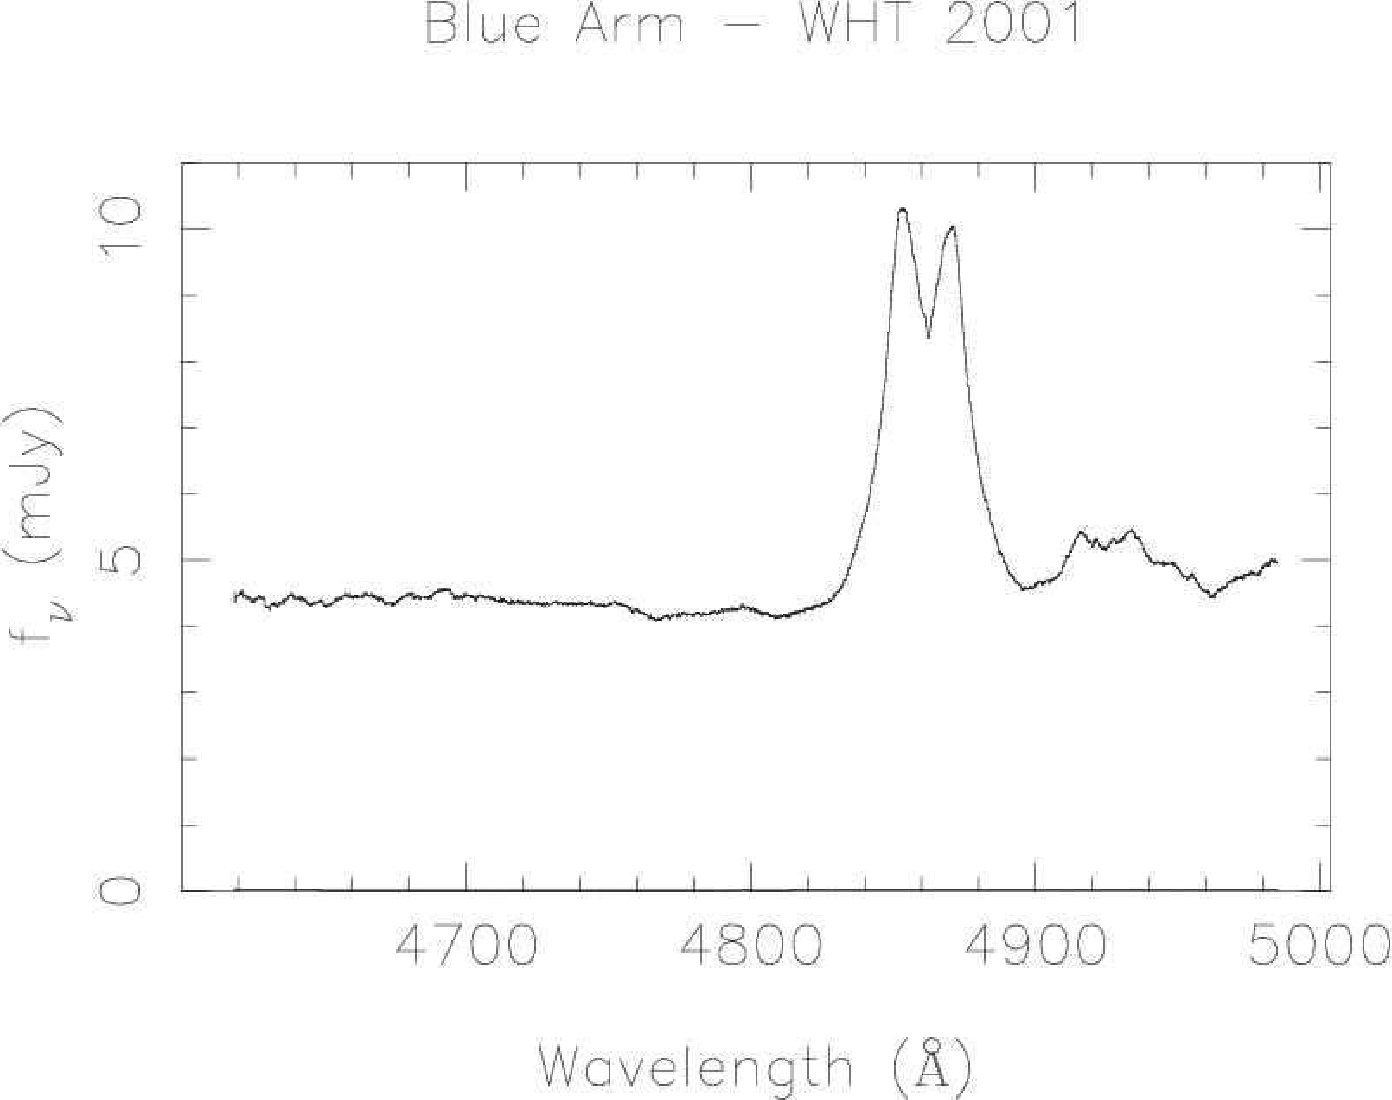
\includegraphics[width=0.78\textwidth]{ugem_wht_hbeta_double_peak.png}
\caption{Observed high-dispersion H$\beta$ profile of the dwarf nova U~Gem
in quiescence. The two maxima on either side of 4861\,\AA\ are the
approaching and receding sides of the rotating accretion disk. The central
depression is resolved directly in the mean WHT/ISIS spectrum. The
instrumental FWHM was 0.42\,\AA, which corresponds to
$R\simeq11{,}600$ and about $26\,\kms$ at H$\beta$. The proposed
$R=5000$ mode would sample the measured peak separation while retaining
survey efficiency. Cropped from Figure~1 of Unda-Sanzana et al. (2006)
\cite{undasanzana2006}.}
\label{fig:dwarf_profile}
\end{figure}

\subsection{Cadence for dwarf novae}

The mission should not treat dwarf novae as isolated targets that receive one
spectrum per year. Sparse imaging first determines the quiescent level and
identifies the outburst onset. Triggered spectroscopy then samples the rise,
maximum and decline. A selected bright subset receives a dense sequence over
at least one binary orbit. The three temporal scales measure recurrence,
thermal-state evolution, and orbital kinematics respectively.

Orbital tomography requires approximately uniform phase coverage. If one
desires $N_\phi$ independent bins, an individual integration should satisfy
\begin{equation}
 t_{\rm exp}\lesssim \frac{P_{\rm orb}}{N_\phi}.
 \label{eq:phase_smear}
\end{equation}
A reference value of $N_\phi=10$ limits phase smearing to one tenth of an
orbit. Detector read noise and readout overhead determine whether this
condition is met for a given source. The observing plan should report the
number of usable phase bins after occultations, rolls and rejected frames.
The monthly and weekly cadences in Table~\ref{tab:target_selection} describe
state sampling. The monthly and weekly cadences do not replace the dense
sequence needed for tomography.

The slitless geometry is an advantage for a population program because the
source and neighboring field objects are modeled jointly in direct and
dispersed images. The geometry is also a risk. A nearby contaminating star may
produce an overlapping trace. A dwarf nova in a crowded field may be lost if the
scene model is based only on a static continuum template. The reduction must
fit the direct image, all available roll angles, the spectral trace,
and the time-dependent source flux in one forward model.

\section{White Dwarfs and Dense-Matter Laboratories}

White dwarfs connect compact-object observations to stellar evolution,
crystallization and the fate of planetary systems. White-dwarf pulsations probe
internal chemical stratification, total mass, rotation and magnetic-field
properties when compared with stellar-structure models
\cite{corsico2019}. The imaging channel provides the long uninterrupted light
curves needed for asteroseismology. The $R=5000$ spectrum provides effective
temperature, surface gravity, atmospheric composition, radial velocity and
metal-pollution diagnostics.

The useful pulsators occupy restricted temperature intervals. Hydrogen
atmosphere ZZ~Ceti stars, helium atmosphere V777~Her stars and hotter
GW~Vir stars require different atmosphere grids and show different ranges of
periods. Spectroscopy first places a target relative to the appropriate
instability strip. The imaging sequence then measures frequencies compared
with the eigenmodes of a model having the measured atmospheric
boundary condition.

Cadence and duration control different parts of the experiment. A sampling
interval $\Delta t$ gives a Nyquist frequency
\begin{equation}
 \nu_{\rm Nyq}=\frac{1}{2\Delta t},
 \qquad
 \delta\nu_{\rm run}\simeq\frac{1}{T_{\rm run}},
 \label{eq:wd_sampling}
\end{equation}
where $T_{\rm run}$ is the uninterrupted duration. Sub-minute imaging
samples short pulsations while a run of many hours resolves nearby modes and
reduces daily aliasing. The proposal must state the photometric precision per
sample and the expected mode-amplitude threshold. A cadence value without
these quantities does not establish an asteroseismic yield.

For a polluted white dwarf, the optical spectrum identifies or constrains
elements such as Ca, Mg, Fe and Si. The interpretation requires diffusion and
accretion models. The telescope does not directly measure the composition of
the disrupted parent body. The spectrum measures atmospheric abundances that are then
translated into parent-body composition using a physical model.

The atmospheric product consists of a calibrated spectrum, effective
temperature, surface gravity, atmospheric class, line abundances and radial
velocity. The interior product consists of pulsation frequencies, amplitudes
and temporal evolution. The separation avoids attributing an interior
measurement to spectroscopy alone. The time-series photometry and the
spectrum are complementary parts of the same white-dwarf experiment.

The resolving power also places a limit on the abundance claim. Strong Ca
features and broad hydrogen or helium profiles are measurable at $R=5000$ for
sufficiently bright stars. Weak blends and detailed abundance patterns often
require higher resolution from a ground-based spectrograph. The space program
should be presented as a homogeneous discovery and atmospheric-characterization
survey followed by high-resolution work on the most informative polluted
systems.

\section{Black-Hole and Neutron-Star Accretion Transients}

Compact accretors that are not detected through a gravitational-wave alert
also produce useful optical and near-infrared time series. Stellar-mass black
hole binaries and neutron-star X-ray binaries show rapid changes in
continuum slope, emission lines and line asymmetry. X-ray and gamma-ray
facilities provide the high-energy trigger while the proposed telescope
measures the lower-energy response. Tidal-disruption events are not included
in the baseline sample because the extended hosts and nuclear positions
create a different slitless-extraction problem.

The optical and near-infrared continuum separates a thermal disk component
from synchrotron emission only when the spectral sequence is combined with
the X-ray state. He~II and the Bowen blend trace irradiation by the
high-energy source. The velocity curves may reveal an irradiated donor in
selected systems, but disk and wind components may shift the measured
centroid. Blue-shifted absorption and evolving line wings provide evidence for
an outflow when the wavelength calibration and comparison epochs exclude a
trace artifact. Repeated imaging adds periodic or quasi-periodic modulation
and ties each spectrum to the accretion state.

The trigger sample should be restricted to systems for which the predicted
optical or near-infrared flux reaches the line-S/N requirement. An X-ray alert
alone does not guarantee a useful spectrum. The target decision requires an
updated counterpart position, extinction estimate, current optical magnitude,
and the expected lifetime of the state. Bright benchmark binaries
calibrate the relation between the high-energy state and the lower-energy
spectrum. Fainter events should enter only when the ETC predicts a measurable
continuum or a specified line flux.

Joint observations distinguish a disk-dominated flare from a jet-dominated
event only when the spectra are combined with multi-band light curves and
external high-energy information. The appendix should therefore describe
the targets as a coordinated-network program, not as a standalone optical
classification survey.

\section{Science-to-Requirement Feasibility}

\begin{table}[H]
\centering
\caption{Reference requirements for the compact-object program. The values are
planning values to be verified by an end-to-end ETC and scene simulation.}
\label{tab:requirements}
\begin{tabularx}{\textwidth}{@{}P{43mm} P{30mm} Y@{}}
\toprule
\textbf{Requirement} & \textbf{Reference value} & \textbf{Reason}\\
\midrule
Wavelength range & $0.2$--$1.5\micron$ & Covers ultraviolet/optical transient
continuum, Balmer and helium lines, and selected NIR transitions. Each detector
channel requires an independent sensitivity budget\\
Point-source resolving power & $R=5000$ & Resolves approximately $60\,\kms$
velocity structure in accretion-disk profiles. Broad transient features are
binned to lower resolution\\
Spectral calibration & Stability set by the velocity error budget & Required
for line-centroid and radial-velocity comparison across epochs\\
ToO response & Goal $<4$ hr, baseline $<12$ hr & Captures early kilonova and
rapid accretion-state evolution\\
Photometric cadence & Sub-minute for selected targets & White-dwarf
pulsations and ultracompact-binary variability\\
Spectroscopic cadence & Minutes to days, event dependent & Separates orbital
modulation from outburst evolution\\
Roll-angle coverage & Two with a scene-dependent third orientation & Controls
overlapping traces without imposing unnecessary ToO overhead\\
PSF stability & Calibrated over each sequence & Enables line-flux extraction
and precise time-series subtraction\\
\bottomrule
\end{tabularx}
\end{table}

\subsection{Spectroscopic ETC implementation}

The initial spectroscopic ETC is implemented as the \texttt{mission\_etc}
package. The numerical kernel remains in \texttt{slitless\_etc.py} while the
user interface separates imaging, isolated-line spectroscopy, template
spectroscopy, cooled mid-infrared imaging and validation. The separation
prevents an AB magnitude, an integrated line flux and a calibrated
$F_\lambda$ spectrum from entering the same calculation without an explicit
observing mode.

The template mode reads an observed-frame spectrum in physical flux units.
The calculation convolves the spectrum with a constant-$R$ Gaussian
line-spread function and samples the result on detector pixels. Source counts,
zodiacal and telescope backgrounds, dark current, read variance and
contamination counts remain separate outputs. Each slitless detector pixel
receives the diffuse background integrated over the complete order-sorting
band. Relative flux calibration and contamination-model residuals are treated
as correlated terms when pixels are combined. The correlated terms do not
decrease as the square root of the number of binned pixels.

The current $R=5000$ settings cover 4300--5100\,\AA,
6200--6900\,\AA\ and $1.0$--$1.5\micron$. Two $R=1000$ settings cover
$0.4$--$1.0\micron$ and $1.0$--$1.5\micron$ for broad transient spectra. The
implemented settings test the compact-object diagnostics and the resolution
trade. The settings do not yet establish continuous sensitivity over the
adopted $0.2$--$1.5\micron$ envelope. Separate ultraviolet throughput and
detector models are required below $0.4\micron$. Additional order-sorting
settings are required between the present $R=5000$ bands.

The compact-red reference calculation gives a point-source
$5\sigma$ H$\alpha$ line limit of
$1.48\times10^{-17}\,\mathrm{erg\,s^{-1}\,cm^{-2}}$ in 1800\,s. The
6200--6900\,\AA\ band gives $3.24\times10^3$ sky electrons in a
2.55-pixel line footprint under the adopted background. The inverse
calculation recovers ${\rm S/N}=5$ to numerical precision. These values use
proposal throughput and detector requirements. The values are not measured
flight performance and will change when component transmission, detector
noise and the point-source line-spread function are measured.

The ETC returns S/N per detector pixel and per combined spectral bin. The
same output provides line-flux uncertainty, centroid precision, a
wavelength-calibration floor and the second velocity moment. A phase-smearing
diagnostic limits each exposure to a specified fraction of the binary period.
A broadband limiting magnitude alone is not an adequate compact-object
feasibility metric.

For an extraction aperture containing $N_{\rm pix}$ pixels, a reference
counting-noise expression is
\begin{equation}
 {\rm S/N} =
 \frac{N_{\rm src}}
 {\left[N_{\rm src}+N_{\rm pix}
 (N_{\rm sky}+N_{\rm dark}+n_{\rm read}\sigma_{\rm read}^2)
 +\sigma_{\rm cont}^2\right]^{1/2}},
 \label{eq:snr_budget}
\end{equation}
where $N_{\rm src}$ is the source count in the fitted spectral bin.
$N_{\rm sky}$ and $N_{\rm dark}$ are the sky and dark counts per pixel.
The number of reads is $n_{\rm read}$ and the read noise is
$\sigma_{\rm read}$. The contamination term $\sigma_{\rm cont}$ includes the
uncertainty of overlapping traces. In slitless data the sky term is set by the
full band-limiting filter recorded by each pixel. Increasing the native
dispersion may therefore reduce the S/N of a broad feature even when the final
spectrum is binned.

For a Gaussian line with integrated flux $F_{\rm line}$ and uncertainty
$\sigma_F$, the line detection statistic is
\begin{equation}
  {\rm S/N}_{\rm line} = \frac{F_{\rm line}}{\sigma_F},
  \qquad
  \sigma_{v,\rm stat} \propto
  \frac{c}{R\,{\rm S/N}_{\rm line}}.
  \label{eq:line_precision}
\end{equation}
The proportionality factor depends on the line profile and sampling. The
proposal should quote the full simulated value rather than assume that the
simple scaling is exact.

The total velocity error must also include a calibration floor,
\begin{equation}
 \sigma_v^2=\sigma_{v,\rm stat}^2+\sigma_{v,\rm wave}^2+
 \sigma_{v,\rm scene}^2+\sigma_{v,\rm model}^2 ,
 \label{eq:velocity_budget}
\end{equation}
where the additional terms arise from the wavelength solution, source
position and contamination and the adopted line model. The requirement on
spectral stability should be stated as a limit on these terms. The phrase
``stable wavelength solution'' is not a verifiable requirement by itself.

The same discipline applies to mission time. The exact integrations in
Table~\ref{tab:target_selection} are planning values until
Equation~\ref{eq:snr_budget} is evaluated for the quiescent and outburst
magnitudes of every benchmark. The proposal should publish a matrix of
continuum S/N, line-flux S/N and overlap survival probability for each source
class. That matrix determines which candidates remain in the baseline and
which become optional targets.

\subsubsection{Observed-template reference cases}

The second ETC stage assigns provenance and a native resolving power to each
observed template. The line-spread calculation applies only the Gaussian
kernel required between the native resolution and the selected mission
setting. A template with lower resolution is not sharpened. The same record
retains the epoch, source state, wavelength frame, flux uncertainty, citation
and public data address.

Figure~\ref{fig:compact_etc_reference} presents reference calculations based
on the LAMOST spectrum of U~Gem at the peak of its 2012 December outburst
\cite{zhi2020} and the ENGRAVE reduction of the AT~2017gfo X-shooter sequence
\cite{pian2017,smartt2017,engrave2019}. The U~Gem H$\alpha$ line reaches an
integrated S/N of 20 in 11.5\,s under the adopted instrument assumptions. The
native LAMOST resolving power is approximately 1800. The result constrains
counting statistics and broad line structure but does not validate
$R=5000$ double-peak recovery.

Three hundred detector-noise realizations of the U~Gem case gave a line
centroid bias of $1.6\,\kms$ and a scatter of $20.0\,\kms$. The median local
Fisher estimate was $6.2\,\kms$. The difference shows that a moment estimator
understates the uncertainty of the structured line profile. The next
validation stage must fit the complete profile and must report the empirical
covariance.

The AT~2017gfo calculation uses one broad-feature interval in each channel.
An integrated S/N of 20 at $0.75\micron$ requires 5.7, 47.7 and 241.5\,s at
1.43, 4.40 and 7.40 days after GW170817. The corresponding $1.25\micron$
exposures are 8.9, 14.5 and 45.0\,s. The values demonstrate the fading-rate
calculation and the optical to near-infrared color evolution. The values do
not include alert latency, slew time, trace overlap or a measured flight
throughput.

\begin{figure}[H]
\centering
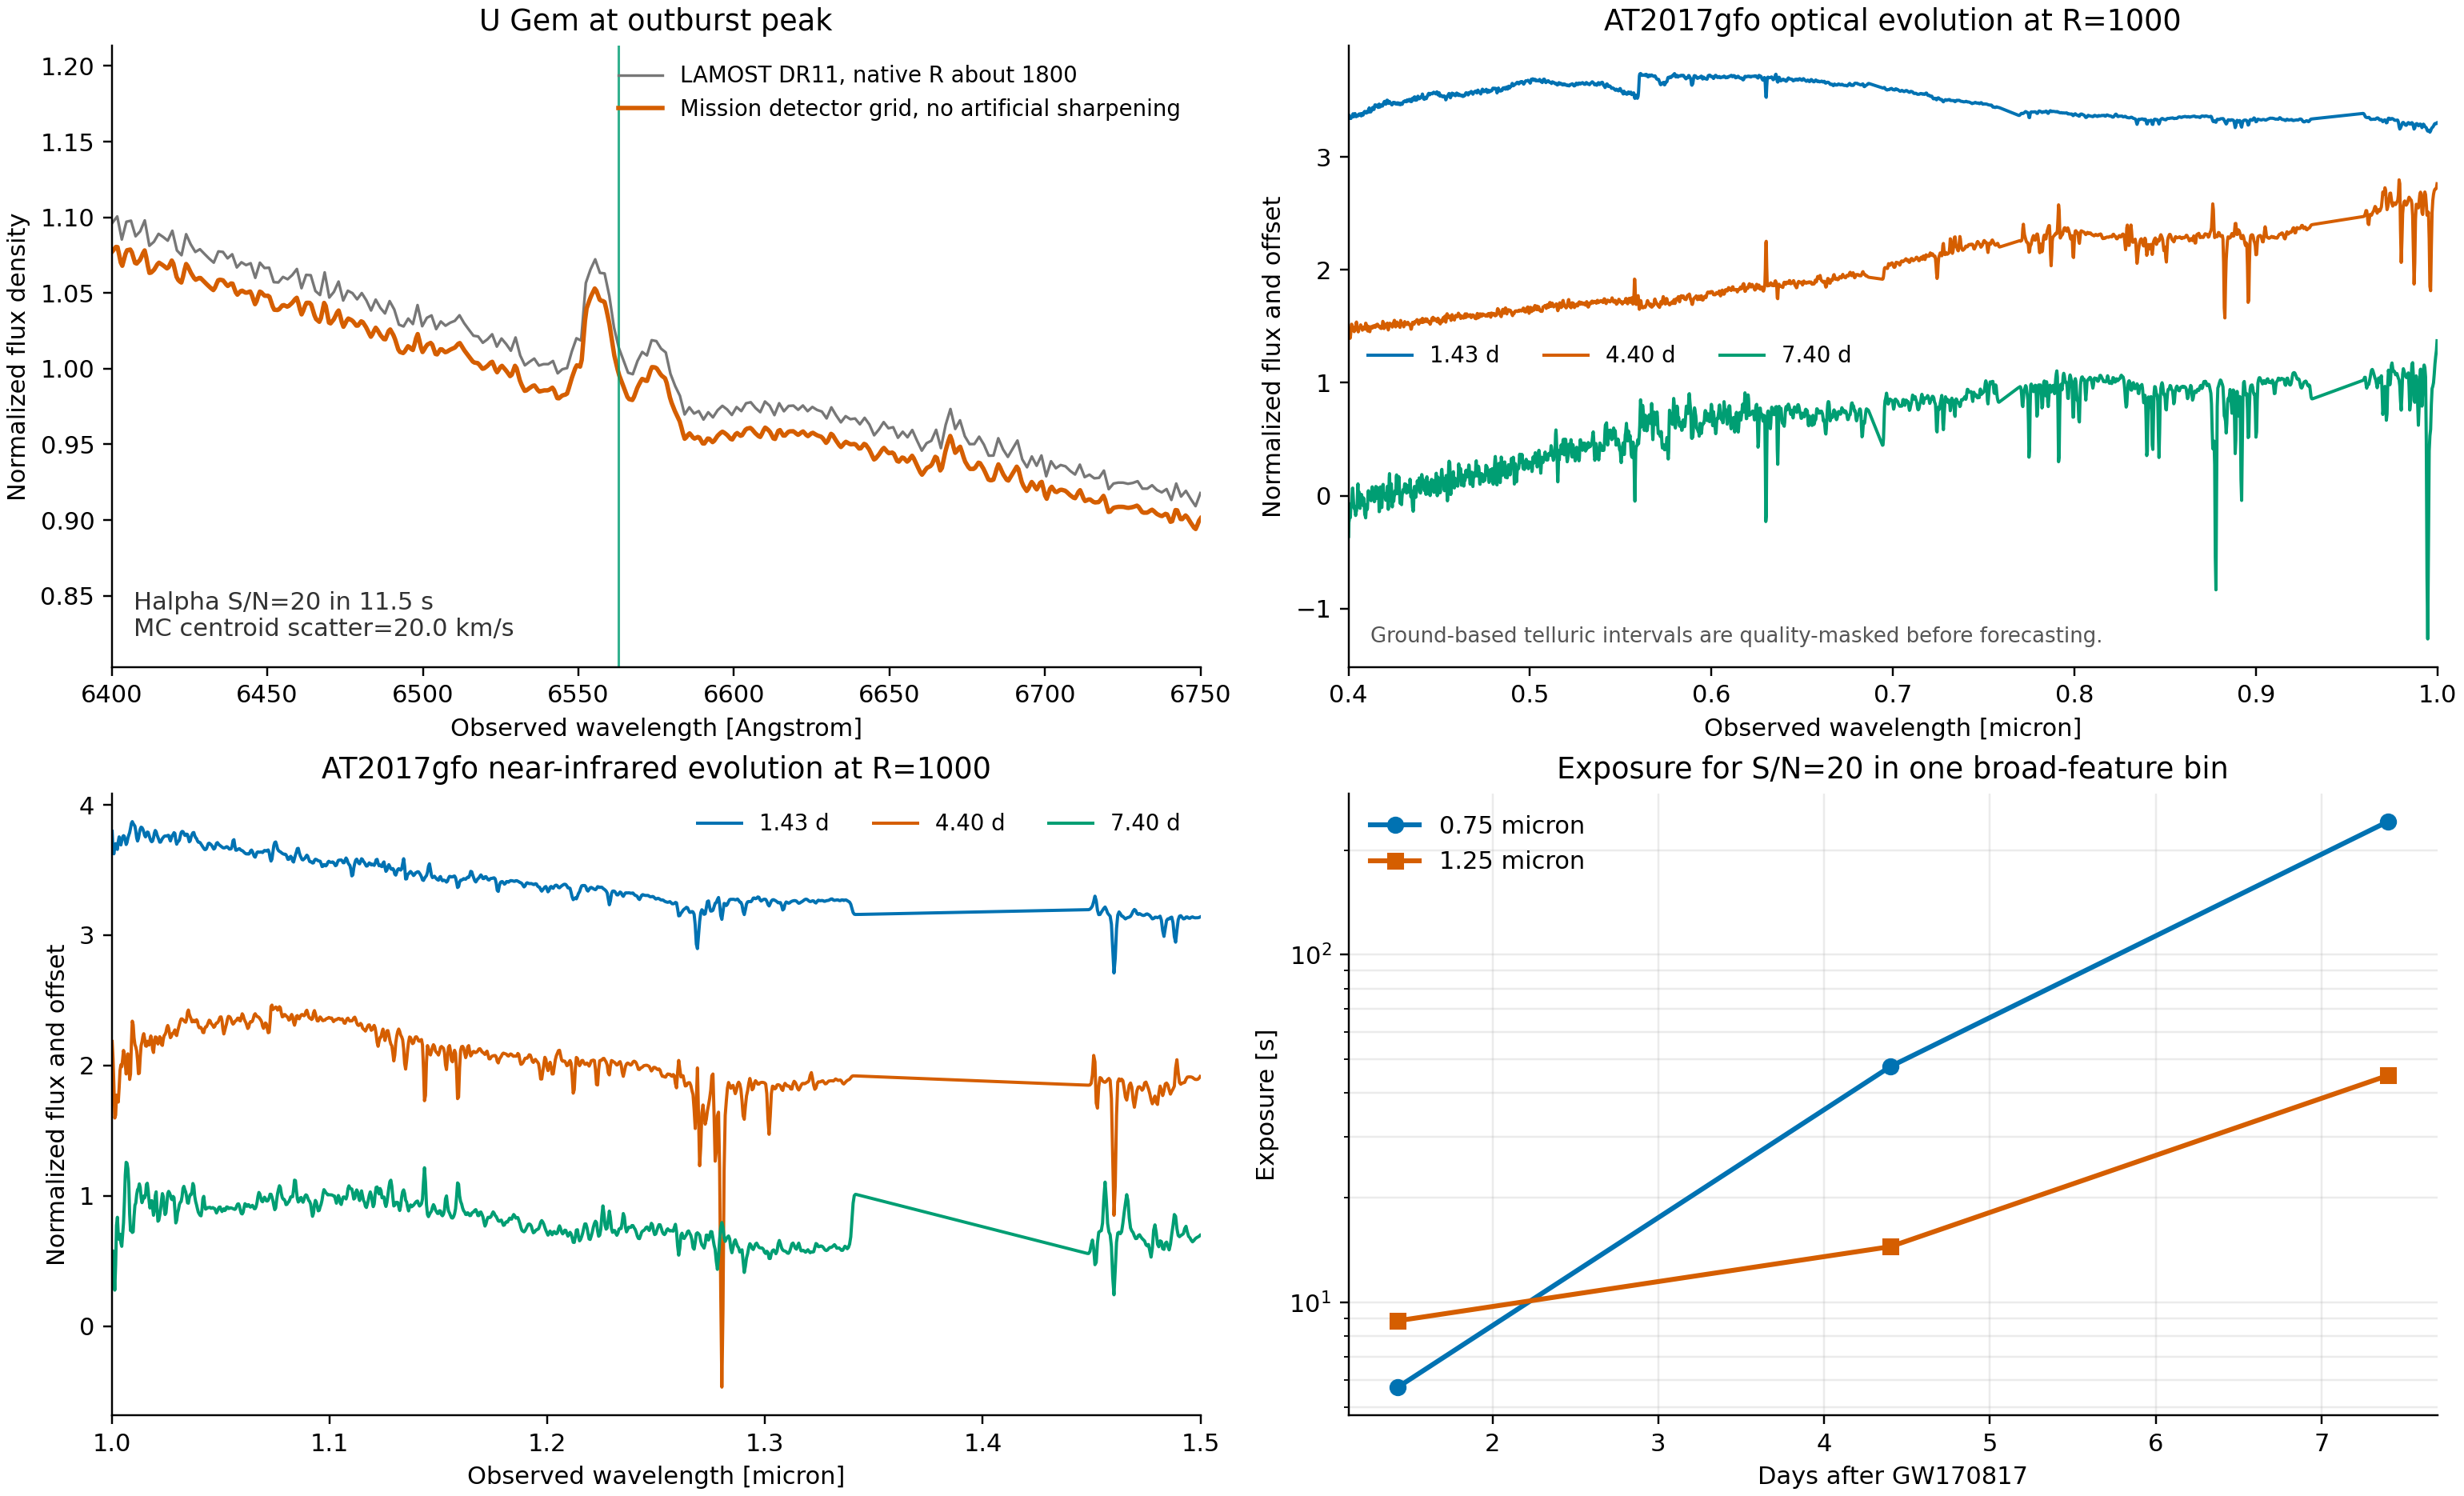
\includegraphics[width=0.99\textwidth]{compact_etc_reference_cases.png}
\caption{Observed-template ETC reference cases. The upper left panel compares
the public LAMOST U~Gem spectrum with the detector-sampled calculation at the
native effective resolution. The other spectral panels use the public
ENGRAVE X-shooter sequence of AT~2017gfo. Known telluric intervals were
excluded before the broad-feature calculation because the ground-based
correction residuals are not intrinsic kilonova structure. Straight segments
across the excluded intervals represent interpolation. The lower right panel
shows the exposure required for an integrated S/N of 20 in a 150\,\AA\
optical interval and a 250\,\AA\ near-infrared interval. All exposure values
use proposal-level throughput and detector assumptions.}
\label{fig:compact_etc_reference}
\end{figure}

\subsubsection{Multi-orientation injection and recovery}

The next calculation tests spectral confusion rather than isolated-source
counting statistics. The direct-image prior contains U~Gem and two nearby
field sources. Each source uses the public LAMOST U~Gem outburst spectrum with
an independent velocity and flux scale. The target receives an injected
velocity of $120\,\kms$. The forward calculation disperses the three sources
onto detector images and adds source shot noise, diffuse background, dark
current and read noise.

The comparison fixes the total science exposure at 60\,s. The single
orientation receives the full 60\,s. The multi-orientation sequence receives
20\,s at each of $0^\circ$, $60^\circ$ and $120^\circ$. A common
direct-image position prior defines the source coordinates. The extraction
then fits all source spectra simultaneously and the recovered U~Gem spectrum
is fitted with the complete H$\alpha$ profile. The profile fit includes a
velocity shift, an amplitude and a linear continuum.

Figure~\ref{fig:compact_scene_recovery} shows the result for 80 independent
detector-noise realizations. All 80 fits converged in both observing
strategies. The single-orientation fit gives a median velocity of
$56.6\,\kms$. The bias is $-63.2\,\kms$ and the empirical scatter is only
$2.6\,\kms$. The small scatter does not indicate an accurate measurement
because the contaminating trace lies along the target trace. Additional
counts do not remove the geometric degeneracy.

The three-orientation fit gives a median velocity of $119.4\,\kms$. The bias
falls to $+1.2\,\kms$ and the empirical scatter is $4.7\,\kms$. Dividing the
exposure among three orientations modestly increases the random error while
the changed projected separation removes the much larger systematic error.
The median diagonal-Fisher estimate is $2.8\,\kms$ for the joint fit. The
empirical scatter must set the velocity requirement because the diagonal
estimate omits covariance among overlapping spectra.

\begin{figure}[H]
\centering
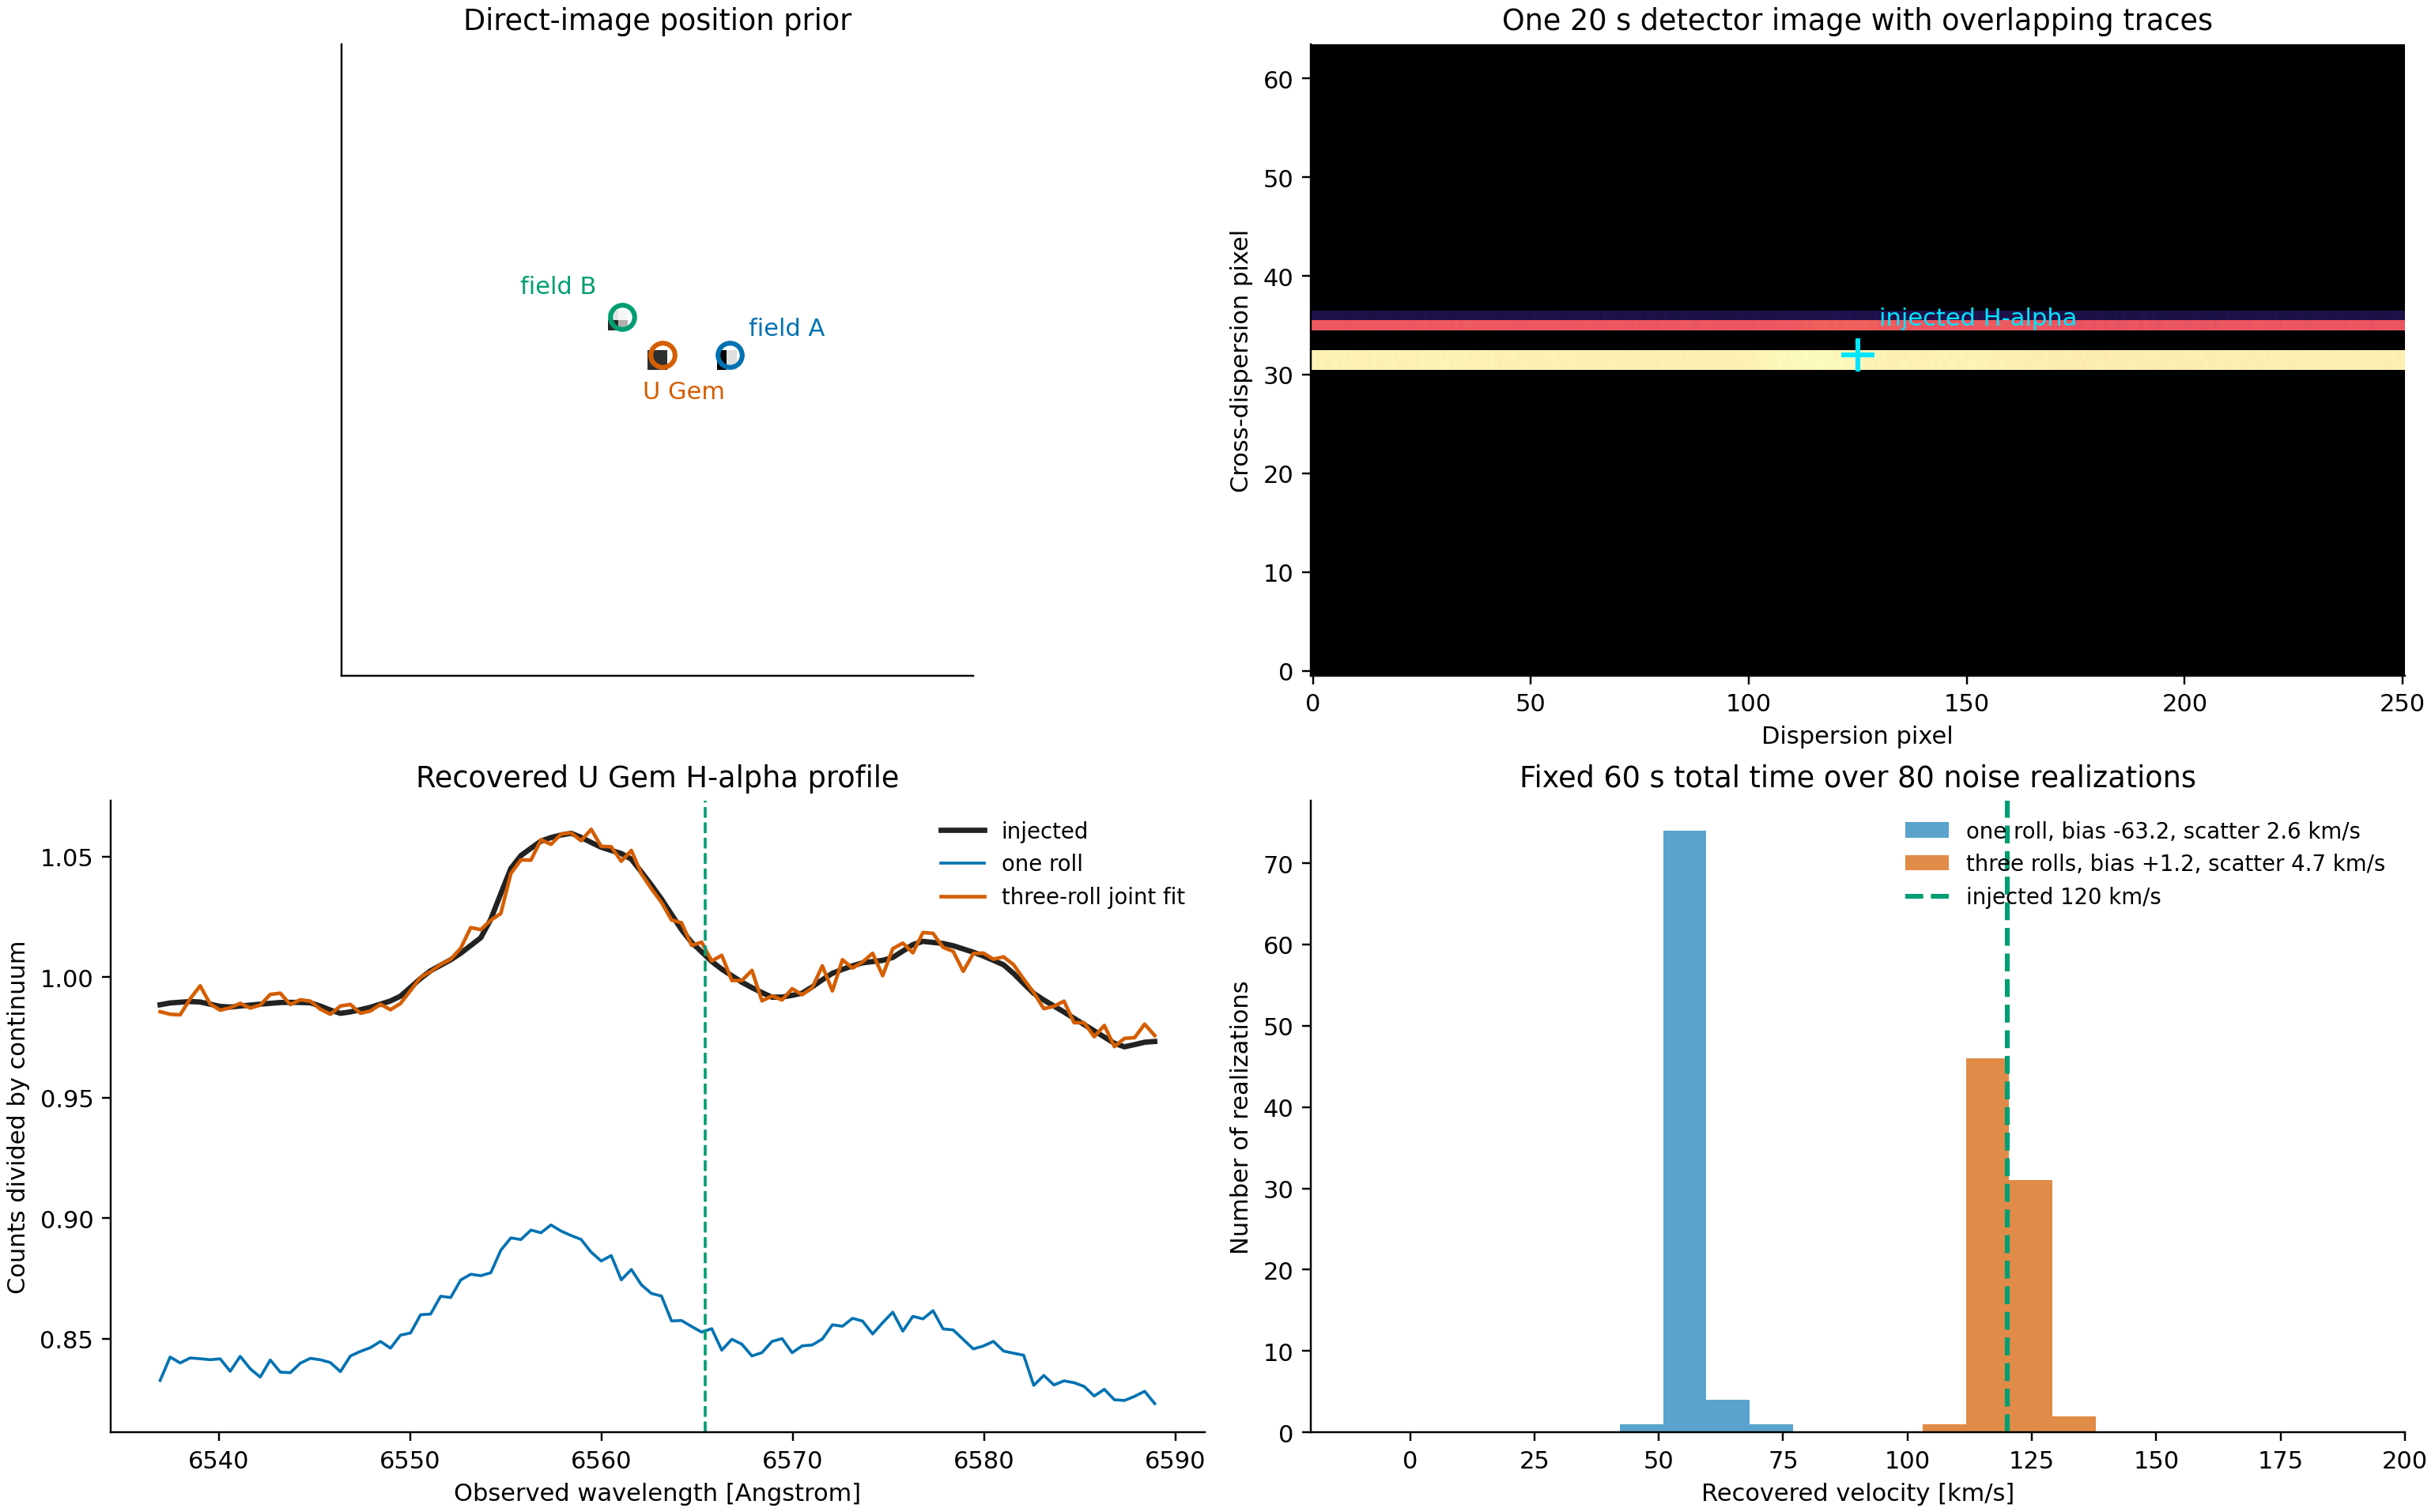
\includegraphics[width=0.99\textwidth]{compact_scene_recovery.png}
\caption{Fixed-time slitless injection and recovery using the public LAMOST
U~Gem spectrum. The upper panels show the direct-image position prior and one
20\,s detector exposure. The lower left panel compares the injected
H$\alpha$ profile with the single-orientation and joint three-orientation
extractions. The lower right panel shows the recovered velocity for 80 noise
realizations. Both observing strategies use 60\,s of total science exposure.
The LAMOST spectrum has an effective resolving power near 1800. The
experiment validates multi-orientation trace separation and does not validate
double-peak recovery at $R=5000$.}
\label{fig:compact_scene_recovery}
\end{figure}

\section{Network Complementarity and Limitations}

The compact-object program is intentionally network based.

\begin{table}[H]
\centering
\caption{Division of labor among complementary facilities.}
\label{tab:network}
\begin{tabularx}{\textwidth}{@{}P{34mm} Y Y@{}}
\toprule
\textbf{Facility class} & \textbf{Primary information} & \textbf{Role of the
3.5 m space telescope}\\
\midrule
Gravitational-wave detectors & Binary masses, distance, tidal information &
Rapid electromagnetic localization and spectral follow-up\\
X-ray and gamma-ray missions & Jet, disk, and high-energy trigger &
Optical/NIR response and host identification\\
Wide-field optical surveys & Discovery and large-area cadence &
High-quality repeated spectra and rapid response\\
Large ground telescopes & Very high-resolution spectroscopy &
Space-stable moderate-resolution time series and early response\\
Deep IR facilities & Faint late-time thermal and spectroscopic information &
Optical/NIR evolution and complementary calibration\\
\bottomrule
\end{tabularx}
\end{table}

A wide gravitational-wave localization region makes spectroscopy inefficient
until an optical counterpart is identified. The mission therefore responds to
a localized counterpart rather than tiling the full gravitational-wave
probability map with $R=5000$ spectra. Kilonova ejecta mass, composition,
opacity, geometry and viewing angle remain degenerate in optical and
near-infrared data. The external gravitational-wave posterior and
radiative-transfer model are part of the inference.

The telescope also does not replace X-ray, gamma-ray, or high-resolution
spectroscopic facilities. The moderate-resolution time series measures a
stable lower-energy response that is difficult to obtain from the ground at
the same cadence. High-resolution spectra remain necessary for weak metal
lines and detailed abundance work. Extended hosts and unrelated sources may
overlap a slitless trace. Every released spectrum must therefore include a
scene-quality flag and the posterior contamination fraction.

White-dwarf interior parameters provide a final example of the division of
labor. The spectrum supplies the atmospheric boundary condition and the
imaging supplies the pulsation frequencies. Stellar models connect those data
to the interior. The proposal should preserve the division of labor in the science
requirements and projected data products.

\section{Required Validation Before Proposal Baseline}

Before this program is treated as a mission-level performance claim, the
following validation products should be completed.

The first validation product is an ETC grid that spans magnitude, line flux,
source state, background, detector channel and roll-dependent contamination
for kilonovae, dwarf novae, white dwarfs and accreting neutron-star or
black-hole binaries. The grid must be based on observed spectral templates.
The second product is a slitless forward simulation that uses direct-image
priors, detector sampling, multiple dispersion orientations, time-dependent
source flux and unrelated field sources. A blinded recovery test should then
measure bias and covariance for injected line profiles and known velocities.

Operational feasibility requires a separate scheduler simulation. The
simulation must begin with a realistic alert stream and must include
classification latency, field of regard, solar avoidance, slew time, roll
availability, guide-star acquisition, downlink and interrupted visits. The
output is a five-year yield that distinguishes public triggers, identified
counterparts, observed targets, spectra with usable line S/N and
science-grade multi-epoch sequences.

Two class-specific demonstrations complete the validation. Archival spectra
and light curves of dwarf novae with known orbital periods should test the
recovery of peak separation, wings, velocity modulation and state changes
after convolution to the proposed instrument. Injected white-dwarf light
curves should test how cadence, gaps and photometric noise change the
recovered pulsation frequencies. The class-specific demonstrations convert the proposed
measurements into traceable performance requirements.

\begin{resultbox}{orange}
\textbf{Recommended proposal position.}
The compact-object program is scientifically credible as a point-source
optical and near-infrared time-domain program. Mission feasibility remains
conditional on the ETC, scene-recovery, scheduler, and yield demonstrations
defined above. The $R=5000$ mode is most valuable for accretion-disk profiles
and should provide lower-resolution binned products for broad transients. The
science claims require joint inference with gravitational-wave, high-energy,
and radiative-transfer information. The program does not require a
mid-infrared instrument and does not claim a direct equation-of-state or
interior measurement from one spectrum.
\end{resultbox}

\section{Summary}

The adopted compact-object baseline is a $0.2$--$1.5\micron$ space-based
slitless spectrograph with $R=5000$, supported by high-cadence imaging and
robotic ToO operations. The point-source nature of compact objects preserves
the native resolution for an isolated trace. Direct images, multiple
orientations and a scene model are still required to control overlap. The
resulting spectra measure velocities, ionization, outflows, disk kinematics,
state changes and transient spectral evolution when the ETC establishes the
required S/N.

The strongest transient case is rapid optical and near-infrared follow-up of
mergers that contain at least one neutron star. Dwarf novae provide a
repeatable population in which line-profile sequences test accretion-disk
instability and binary dynamics. White dwarfs provide a long-baseline program
in which atmospheric spectroscopy and asteroseismology jointly probe cooling,
crystallization, and remnant planetary systems. The three experiments share a
detector but place significantly different requirements on cadence,
resolution, calibration and mission operations.

\begin{thebibliography}{99}

\bibitem{abbott2017}
B.~P. Abbott et al., ``GW170817: Observation of gravitational waves from a
binary neutron star inspiral,'' \emph{Phys. Rev. Lett.} 119, 161101 (2017),
\href{https://doi.org/10.1103/PhysRevLett.119.161101}{doi:10.1103/PhysRevLett.119.161101}.

\bibitem{arcavi2017}
I.~Arcavi et al., ``Optical emission from a kilonova following a
gravitational-wave-detected neutron-star merger,'' \emph{Nature} 551, 64--66
(2017), \href{https://doi.org/10.1038/nature24291}{doi:10.1038/nature24291}.

\bibitem{tanaka2017}
M.~Tanaka et al., ``Kilonova from post-merger ejecta as an optical and
near-infrared counterpart of GW170817,'' \emph{Publ. Astron. Soc. Japan} 69,
102 (2017), \href{https://doi.org/10.1093/pasj/psx121}{doi:10.1093/pasj/psx121}.

\bibitem{watson2019}
D.~Watson et al., ``Identification of strontium in the merger of two neutron
stars,'' \emph{Nature} 574, 497--500 (2019),
\href{https://doi.org/10.1038/s41586-019-1676-3}{doi:10.1038/s41586-019-1676-3}.

\bibitem{pian2017}
E.~Pian et al., ``Spectroscopic identification of r-process nucleosynthesis
in a double neutron-star merger,'' \emph{Nature} 551, 67--70 (2017),
\href{https://doi.org/10.1038/nature24298}{doi:10.1038/nature24298}.

\bibitem{smartt2017}
S.~J. Smartt et al., ``A kilonova as the electromagnetic counterpart to a
gravitational-wave source,'' \emph{Nature} 551, 75--79 (2017),
\href{https://doi.org/10.1038/nature24303}{doi:10.1038/nature24303}.

\bibitem{engrave2019}
ENGRAVE Collaboration, ``AT2017gfo data release,'' public X-shooter spectral
products (2019),
\href{https://www.engrave-eso.org/AT2017gfo-Data-Release/}{ENGRAVE data release}.

\bibitem{chornock2017}
R.~Chornock et al., ``The electromagnetic counterpart of the binary neutron
star merger LIGO/Virgo GW170817. IV. Detection of near-infrared signatures of
r-process nucleosynthesis with Gemini-South,'' \emph{Astrophys. J. Lett.} 848,
L19 (2017),
\href{https://doi.org/10.3847/2041-8213/aa905c}{doi:10.3847/2041-8213/aa905c}.

\bibitem{kim2016kmtnet}
S.-L. Kim et al., ``KMTNet: A network of 1.6 m wide-field optical telescopes
installed at three southern observatories,'' \emph{J. Korean Astron. Soc.} 49,
37--44 (2016),
\href{https://doi.org/10.5303/JKAS.2016.49.1.37}{doi:10.5303/JKAS.2016.49.1.37}.

\bibitem{brown2018ksp}
S.~Brown et al., ``High-cadence multi-color observations of the dwarf nova
KSP-OT-201503a by the KMTNet Supernova Program,'' \emph{Astrophys. J.} 860,
21 (2018),
\href{https://doi.org/10.3847/1538-4357/aabfe2}{doi:10.3847/1538-4357/aabfe2}.

\bibitem{lee2019ksp}
Y.~Lee et al., ``KSP-OT-201611a: A distant Population II dwarf nova candidate
discovered by the KMTNet Supernova Program,'' \emph{Astrophys. J.} 880, 109
(2019),
\href{https://doi.org/10.3847/1538-4357/ab2985}{doi:10.3847/1538-4357/ab2985}.

\bibitem{lee2022ksp}
Y.~Lee et al., ``Discovery of a short-period and unusually helium-deficient
dwarf nova KSP-OT-201701a by the KMTNet Supernova Program,''
\emph{Astrophys. J. Lett.} 925, L22 (2022),
\href{https://doi.org/10.3847/2041-8213/ac4c41}{doi:10.3847/2041-8213/ac4c41}.

\bibitem{lee2024ksp}
Y.~Lee et al., ``Helium-deficient ER UMa-type dwarf nova below the period
minimum with a hot secondary,'' \emph{Astrophys. J.} 964, 186 (2024),
\href{https://doi.org/10.3847/1538-4357/ad25ff}{doi:10.3847/1538-4357/ad25ff}.

\bibitem{kim2026ksp}
S.~C. Kim et al., ``A new WZ Sagittae-type dwarf nova KSP-OT-202104a near the
period minimum from the KMTNet Supernova Program,'' \emph{Astron. J.} 172, 1
(2026),
\href{https://doi.org/10.3847/1538-3881/ae6b7f}{doi:10.3847/1538-3881/ae6b7f}.

\bibitem{lasota2001}
J.-P. Lasota, ``The disc instability model of dwarf novae and low-mass X-ray
binary transients,'' \emph{New Astron. Rev.} 45, 449--508 (2001),
\href{https://doi.org/10.1016/S1387-6473(01)00112-9}{doi:10.1016/S1387-6473(01)00112-9}.

\bibitem{warner1995}
B.~Warner, \emph{Cataclysmic Variable Stars}, Cambridge University Press
(1995), \href{https://doi.org/10.1017/CBO9780511586491}{doi:10.1017/CBO9780511586491}.

\bibitem{horne1986}
K.~Horne and T.~R. Marsh, ``Emission-line formation in accretion discs,''
\emph{Mon. Not. R. Astron. Soc.} 218, 761--773 (1986),
\href{https://doi.org/10.1093/mnras/218.4.761}{doi:10.1093/mnras/218.4.761}.

\bibitem{corsico2019}
A.~H. Córsico, L.~G. Althaus, M.~M. Miller Bertolami, and S.~O. Kepler,
``Pulsating white dwarfs: new insights,'' \emph{Astron. Astrophys. Rev.} 27,
7 (2019),
\href{https://doi.org/10.1007/s00159-019-0118-4}{doi:10.1007/s00159-019-0118-4}.

\bibitem{barros2007}
S.~C.~C. Barros et al., ``ULTRACAM photometry of the ultracompact binaries
V407 Vul and HM Cnc,'' \emph{Mon. Not. R. Astron. Soc.} 374, 1334--1346
(2007),
\href{https://doi.org/10.1111/j.1365-2966.2006.11244.x}{doi:10.1111/j.1365-2966.2006.11244.x}.

\bibitem{stella1987}
L.~Stella, W.~Priedhorsky, and N.~E. White, ``The discovery of a 685 second
orbital period from the X-ray source 4U 1820$-$30 in the globular cluster
NGC 6624,'' \emph{Astrophys. J. Lett.} 312, L17--L21 (1987),
\href{https://doi.org/10.1086/184811}{doi:10.1086/184811}.

\bibitem{zhi2020}
Q.-J. Zhi et al., ``Spectroscopic properties of the dwarf nova-type
cataclysmic variables observed by LAMOST,'' \emph{Publ. Astron. Soc. Japan}
72, 76 (2020),
\href{https://doi.org/10.1093/pasj/psaa065}{doi:10.1093/pasj/psaa065}.

\bibitem{eso1733j}
European Southern Observatory, ``X-shooter spectra montage of kilonova in
NGC 4993,'' ESO image eso1733j (2017),
\href{https://www.eso.org/public/images/eso1733j/}{ESO public image archive}.

\bibitem{rittercv}
H.~Ritter and U.~Kolb, \emph{Catalogue of Cataclysmic Binaries, Low-Mass
X-ray Binaries and Related Objects}, 7th edition, release 7.21 (2014),
NASA HEASARC RITTERCV database,
\href{https://heasarc.gsfc.nasa.gov/w3browse/all/rittercv.html}{public catalog}.

\bibitem{lvkalerts}
LIGO Scientific Collaboration, Virgo Collaboration, and KAGRA Collaboration,
``Public alerts user guide,'' IGWN,
\href{https://emfollow.docs.ligo.org/userguide/}{public alert documentation}.

\bibitem{undasanzana2006}
E.~Unda-Sanzana, T.~R. Marsh, and L.~Morales-Rueda, ``Optical spectroscopy
of the dwarf nova U Geminorum,'' \emph{Mon. Not. R. Astron. Soc.} 369,
805--818 (2006),
\href{https://doi.org/10.1111/j.1365-2966.2006.10336.x}{doi:10.1111/j.1365-2966.2006.10336.x}.

\end{thebibliography}

\end{document}
